\documentclass[1p]{elsarticle_modified}
%\bibliographystyle{elsarticle-num}

%\usepackage[colorlinks]{hyperref}
%\usepackage{abbrmath_seonhwa} %\Abb, \Ascr, \Acal ,\Abf, \Afrak
\usepackage{amsfonts}
\usepackage{amssymb}
\usepackage{amsmath}
\usepackage{amsthm}
\usepackage{scalefnt}
\usepackage{amsbsy}
\usepackage{kotex}
\usepackage{caption}
\usepackage{subfig}
\usepackage{color}
\usepackage{graphicx}
\usepackage{xcolor} %% white, black, red, green, blue, cyan, magenta, yellow
\usepackage{float}
\usepackage{setspace}
\usepackage{hyperref}

\usepackage{tikz}
\usetikzlibrary{arrows}

\usepackage{multirow}
\usepackage{array} % fixed length table
\usepackage{hhline}

%%%%%%%%%%%%%%%%%%%%%
\makeatletter
\renewcommand*\env@matrix[1][\arraystretch]{%
	\edef\arraystretch{#1}%
	\hskip -\arraycolsep
	\let\@ifnextchar\new@ifnextchar
	\array{*\c@MaxMatrixCols c}}
\makeatother %https://tex.stackexchange.com/questions/14071/how-can-i-increase-the-line-spacing-in-a-matrix
%%%%%%%%%%%%%%%

\usepackage[normalem]{ulem}

\newcommand{\msout}[1]{\ifmmode\text{\sout{\ensuremath{#1}}}\else\sout{#1}\fi}
%SOURCE: \msout is \stkout macro in https://tex.stackexchange.com/questions/20609/strikeout-in-math-mode

\newcommand{\cancel}[1]{
	\ifmmode
	{\color{red}\msout{#1}}
	\else
	{\color{red}\sout{#1}}
	\fi
}

\newcommand{\add}[1]{
	{\color{blue}\uwave{#1}}
}

\newcommand{\replace}[2]{
	\ifmmode
	{\color{red}\msout{#1}}{\color{blue}\uwave{#2}}
	\else
	{\color{red}\sout{#1}}{\color{blue}\uwave{#2}}
	\fi
}

\newcommand{\Sol}{\mathcal{S}} %segment
\newcommand{\D}{D} %diagram
\newcommand{\A}{\mathcal{A}} %arc


%%%%%%%%%%%%%%%%%%%%%%%%%%%%%5 test

\def\sl{\operatorname{\textup{SL}}(2,\Cbb)}
\def\psl{\operatorname{\textup{PSL}}(2,\Cbb)}
\def\quan{\mkern 1mu \triangleright \mkern 1mu}

\theoremstyle{definition}
\newtheorem{thm}{Theorem}[section]
\newtheorem{prop}[thm]{Proposition}
\newtheorem{lem}[thm]{Lemma}
\newtheorem{ques}[thm]{Question}
\newtheorem{cor}[thm]{Corollary}
\newtheorem{defn}[thm]{Definition}
\newtheorem{exam}[thm]{Example}
\newtheorem{rmk}[thm]{Remark}
\newtheorem{alg}[thm]{Algorithm}

\newcommand{\I}{\sqrt{-1}}
\begin{document}

%\begin{frontmatter}
%
%\title{Boundary parabolic representations of knots up to 8 crossings}
%
%%% Group authors per affiliation:
%\author{Yunhi Cho} 
%\address{Department of Mathematics, University of Seoul, Seoul, Korea}
%\ead{yhcho@uos.ac.kr}
%
%
%\author{Seonhwa Kim} %\fnref{s_kim}}
%\address{Center for Geometry and Physics, Institute for Basic Science, Pohang, 37673, Korea}
%\ead{ryeona17@ibs.re.kr}
%
%\author{Hyuk Kim}
%\address{Department of Mathematical Sciences, Seoul National University, Seoul 08826, Korea}
%\ead{hyukkim@snu.ac.kr}
%
%\author{Seokbeom Yoon}
%\address{Department of Mathematical Sciences, Seoul National University, Seoul, 08826,  Korea}
%\ead{sbyoon15@snu.ac.kr}
%
%\begin{abstract}
%We find all boundary parabolic representation of knots up to 8 crossings.
%
%\end{abstract}
%\begin{keyword}
%    \MSC[2010] 57M25 
%\end{keyword}
%
%\end{frontmatter}

%\linenumbers
%\tableofcontents
%
\newcommand\colored[1]{\textcolor{white}{\rule[-0.35ex]{0.8em}{1.4ex}}\kern-0.8em\color{red} #1}%
%\newcommand\colored[1]{\textcolor{white}{ #1}\kern-2.17ex	\textcolor{white}{ #1}\kern-1.81ex	\textcolor{white}{ #1}\kern-2.15ex\color{red}#1	}

{\Large $\underline{12a_{0961}~(K12a_{0961})}$}

\setlength{\tabcolsep}{10pt}
\renewcommand{\arraystretch}{1.6}
\vspace{1cm}\begin{tabular}{m{100pt}>{\centering\arraybackslash}m{274pt}}
\multirow{5}{120pt}{
	\centering
	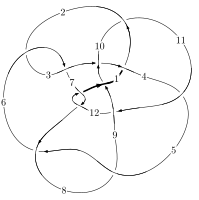
\includegraphics[width=112pt]{../../../GIT/diagram.site/Diagrams/png/1762_12a_0961.png}\\
\ \ \ A knot diagram\footnotemark}&
\allowdisplaybreaks
\textbf{Linearized knot diagam} \\
\cline{2-2}
 &
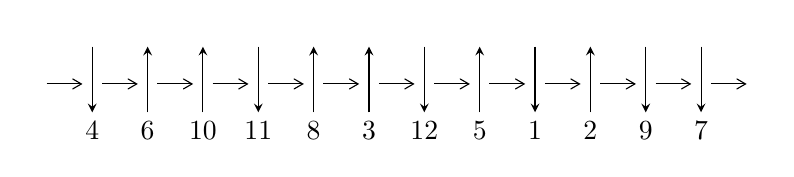
\begin{tikzpicture}[x=20pt, y=17pt]
	% nodes
	\node (C0) at (0, 0) {};
	\node (C1) at (1, 0) {};
	\node (C1U) at (1, +1) {};
	\node (C1D) at (1, -1) {4};

	\node (C2) at (2, 0) {};
	\node (C2U) at (2, +1) {};
	\node (C2D) at (2, -1) {6};

	\node (C3) at (3, 0) {};
	\node (C3U) at (3, +1) {};
	\node (C3D) at (3, -1) {10};

	\node (C4) at (4, 0) {};
	\node (C4U) at (4, +1) {};
	\node (C4D) at (4, -1) {11};

	\node (C5) at (5, 0) {};
	\node (C5U) at (5, +1) {};
	\node (C5D) at (5, -1) {8};

	\node (C6) at (6, 0) {};
	\node (C6U) at (6, +1) {};
	\node (C6D) at (6, -1) {3};

	\node (C7) at (7, 0) {};
	\node (C7U) at (7, +1) {};
	\node (C7D) at (7, -1) {12};

	\node (C8) at (8, 0) {};
	\node (C8U) at (8, +1) {};
	\node (C8D) at (8, -1) {5};

	\node (C9) at (9, 0) {};
	\node (C9U) at (9, +1) {};
	\node (C9D) at (9, -1) {1};

	\node (C10) at (10, 0) {};
	\node (C10U) at (10, +1) {};
	\node (C10D) at (10, -1) {2};

	\node (C11) at (11, 0) {};
	\node (C11U) at (11, +1) {};
	\node (C11D) at (11, -1) {9};

	\node (C12) at (12, 0) {};
	\node (C12U) at (12, +1) {};
	\node (C12D) at (12, -1) {7};
	\node (C13) at (13, 0) {};

	% arrows
	\draw[->,>={angle 60}]
	(C0) edge (C1) (C1) edge (C2) (C2) edge (C3) (C3) edge (C4) (C4) edge (C5) (C5) edge (C6) (C6) edge (C7) (C7) edge (C8) (C8) edge (C9) (C9) edge (C10) (C10) edge (C11) (C11) edge (C12) (C12) edge (C13) ;	\draw[->,>=stealth]
	(C1U) edge (C1D) (C2D) edge (C2U) (C3D) edge (C3U) (C4U) edge (C4D) (C5D) edge (C5U) (C6D) edge (C6U) (C7U) edge (C7D) (C8D) edge (C8U) (C9U) edge (C9D) (C10D) edge (C10U) (C11U) edge (C11D) (C12U) edge (C12D) ;
	\end{tikzpicture} \\
\hhline{~~} \\& 
\textbf{Solving Sequence} \\ \cline{2-2} 
 &
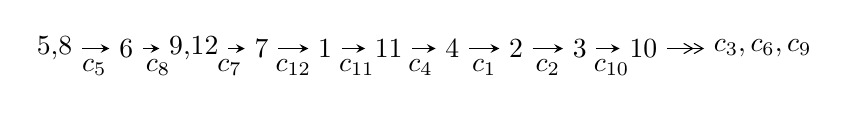
\begin{tikzpicture}[x=23pt, y=7pt]
	% node
	\node (A0) at (-1/8, 0) {5,8};
	\node (A1) at (1, 0) {6};
	\node (A2) at (33/16, 0) {9,12};
	\node (A3) at (25/8, 0) {7};
	\node (A4) at (33/8, 0) {1};
	\node (A5) at (41/8, 0) {11};
	\node (A6) at (49/8, 0) {4};
	\node (A7) at (57/8, 0) {2};
	\node (A8) at (65/8, 0) {3};
	\node (A9) at (73/8, 0) {10};
	\node (C1) at (1/2, -1) {$c_{5}$};
	\node (C2) at (3/2, -1) {$c_{8}$};
	\node (C3) at (21/8, -1) {$c_{7}$};
	\node (C4) at (29/8, -1) {$c_{12}$};
	\node (C5) at (37/8, -1) {$c_{11}$};
	\node (C6) at (45/8, -1) {$c_{4}$};
	\node (C7) at (53/8, -1) {$c_{1}$};
	\node (C8) at (61/8, -1) {$c_{2}$};
	\node (C9) at (69/8, -1) {$c_{10}$};
	\node (A10) at (11, 0) {$c_{3},c_{6},c_{9}$};

	% edge
	\draw[->,>=stealth]	
	(A0) edge (A1) (A1) edge (A2) (A2) edge (A3) (A3) edge (A4) (A4) edge (A5) (A5) edge (A6) (A6) edge (A7) (A7) edge (A8) (A8) edge (A9) ;
	\draw[->>,>={angle 60}]	
	(A9) edge (A10);
\end{tikzpicture} \\ 

\end{tabular} \\

\footnotetext{
The image of knot diagram is generated by the software ``\textbf{Draw programme}" developed by Andrew Bartholomew(\url{http://www.layer8.co.uk/maths/draw/index.htm\#Running-draw}), where we modified some parts for our purpose(\url{https://github.com/CATsTAILs/LinksPainter}).
}\phantom \\ \newline 
\centering \textbf{Ideals for irreducible components\footnotemark of $X_{\text{par}}$} 
 
\begin{align*}
I^u_{1}&=\langle 
1.64373\times10^{1346} u^{188}-4.72952\times10^{1346} u^{187}+\cdots+1.82447\times10^{1347} b-4.68882\times10^{1347},\\
\phantom{I^u_{1}}&\phantom{= \langle  }4.30137\times10^{1350} u^{188}-1.12458\times10^{1351} u^{187}+\cdots+4.29740\times10^{1351} a+1.84917\times10^{1355},\\
\phantom{I^u_{1}}&\phantom{= \langle  }u^{189}-3 u^{188}+\cdots-829201 u+94217\rangle \\
I^u_{2}&=\langle 
6.01544\times10^{80} u^{50}+4.68574\times10^{81} u^{49}+\cdots+2.58939\times10^{81} b-1.94635\times10^{81},\\
\phantom{I^u_{2}}&\phantom{= \langle  }-1.83690\times10^{80} u^{50}-2.22203\times10^{81} u^{49}+\cdots+7.12083\times10^{81} a-2.81314\times10^{82},\;u^{51}+8 u^{50}+\cdots-4 u+1\rangle \\
\\
\end{align*}
\raggedright * 2 irreducible components of $\dim_{\mathbb{C}}=0$, with total 240 representations.\\
\footnotetext{All coefficients of polynomials are rational numbers. But the coefficients are sometimes approximated in decimal forms when there is not enough margin.}
\newpage
\renewcommand{\arraystretch}{1}
\centering \section*{I. $I^u_{1}= \langle 1.64\times10^{1346} u^{188}-4.73\times10^{1346} u^{187}+\cdots+1.82\times10^{1347} b-4.69\times10^{1347},\;4.30\times10^{1350} u^{188}-1.12\times10^{1351} u^{187}+\cdots+4.30\times10^{1351} a+1.85\times10^{1355},\;u^{189}-3 u^{188}+\cdots-829201 u+94217 \rangle$}
\flushleft \textbf{(i) Arc colorings}\\
\begin{tabular}{m{7pt} m{180pt} m{7pt} m{180pt} }
\flushright $a_{5}=$&$\begin{pmatrix}1\\0\end{pmatrix}$ \\
\flushright $a_{8}=$&$\begin{pmatrix}0\\u\end{pmatrix}$ \\
\flushright $a_{6}=$&$\begin{pmatrix}1\\- u^2\end{pmatrix}$ \\
\flushright $a_{9}=$&$\begin{pmatrix}u\\u\end{pmatrix}$ \\
\flushright $a_{12}=$&$\begin{pmatrix}-0.100092 u^{188}+0.261689 u^{187}+\cdots+23563.9 u-4303.00\\-0.0900934 u^{188}+0.259228 u^{187}+\cdots-13005.5 u+2.56997\end{pmatrix}$ \\
\flushright $a_{7}=$&$\begin{pmatrix}-0.0593610 u^{188}+0.186224 u^{187}+\cdots-18020.1 u+1064.13\\-0.0376884 u^{188}+0.100062 u^{187}+\cdots+18573.7 u-2940.42\end{pmatrix}$ \\
\flushright $a_{1}=$&$\begin{pmatrix}0.245622 u^{188}-0.680258 u^{187}+\cdots+16419.8 u+1748.61\\0.203510 u^{188}-0.550514 u^{187}+\cdots+1098.87 u+2932.52\end{pmatrix}$ \\
\flushright $a_{11}=$&$\begin{pmatrix}-0.110635 u^{188}+0.276420 u^{187}+\cdots+45454.3 u-6897.31\\-0.100636 u^{188}+0.273958 u^{187}+\cdots+8884.88 u-2591.75\end{pmatrix}$ \\
\flushright $a_{4}=$&$\begin{pmatrix}-0.0238419 u^{188}+0.144100 u^{187}+\cdots-101667. u+11364.6\\-0.0134360 u^{188}+0.0914865 u^{187}+\cdots-76593.3 u+8566.77\end{pmatrix}$ \\
\flushright $a_{2}=$&$\begin{pmatrix}0.0114209 u^{188}+0.142231 u^{187}+\cdots-180966. u+21035.3\\-0.0292937 u^{188}+0.210185 u^{187}+\cdots-140476. u+15792.6\end{pmatrix}$ \\
\flushright $a_{3}=$&$\begin{pmatrix}-0.00807546 u^{188}+0.184150 u^{187}+\cdots-176170. u+20199.2\\-0.0387995 u^{188}+0.219960 u^{187}+\cdots-128573. u+14231.5\end{pmatrix}$ \\
\flushright $a_{10}=$&$\begin{pmatrix}0.209824 u^{188}-0.701328 u^{187}+\cdots+141674. u-13437.5\\0.162003 u^{188}-0.577950 u^{187}+\cdots+152208. u-15269.2\end{pmatrix}$\\&\end{tabular}
\flushleft \textbf{(ii) Obstruction class $= -1$}\\~\\
\flushleft \textbf{(iii) Cusp Shapes $= -0.149815 u^{188}+0.540340 u^{187}+\cdots-154988. u+16041.2$}\\~\\
\newpage\renewcommand{\arraystretch}{1}
\flushleft \textbf{(iv) u-Polynomials at the component}\newline \\
\begin{tabular}{m{50pt}|m{274pt}}
Crossings & \hspace{64pt}u-Polynomials at each crossing \\
\hline $$\begin{aligned}c_{1}\end{aligned}$$&$\begin{aligned}
&u^{189}-19 u^{188}+\cdots+26 u+1
\end{aligned}$\\
\hline $$\begin{aligned}c_{2},c_{6}\end{aligned}$$&$\begin{aligned}
&8(8 u^{189}+40 u^{188}+\cdots-30029 u-2617)
\end{aligned}$\\
\hline $$\begin{aligned}c_{3}\end{aligned}$$&$\begin{aligned}
&8(8 u^{189}-48 u^{188}+\cdots-42 u-1)
\end{aligned}$\\
\hline $$\begin{aligned}c_{4}\end{aligned}$$&$\begin{aligned}
&u^{189}-8 u^{188}+\cdots-12981419408 u+1387228888
\end{aligned}$\\
\hline $$\begin{aligned}c_{5},c_{8}\end{aligned}$$&$\begin{aligned}
&u^{189}+3 u^{188}+\cdots-829201 u-94217
\end{aligned}$\\
\hline $$\begin{aligned}c_{7},c_{12}\end{aligned}$$&$\begin{aligned}
&u^{189}+63 u^{187}+\cdots-2533599 u-3861113
\end{aligned}$\\
\hline $$\begin{aligned}c_{9}\end{aligned}$$&$\begin{aligned}
&u^{189}-3 u^{188}+\cdots-223100552 u+9191768
\end{aligned}$\\
\hline $$\begin{aligned}c_{10}\end{aligned}$$&$\begin{aligned}
&8(8 u^{189}-88 u^{188}+\cdots-28473 u+4057)
\end{aligned}$\\
\hline $$\begin{aligned}c_{11}\end{aligned}$$&$\begin{aligned}
&64(64 u^{189}+1376 u^{188}+\cdots+45382 u+131644)
\end{aligned}$\\
\hline
\end{tabular}\\~\\
\newpage\renewcommand{\arraystretch}{1}
\flushleft \textbf{(v) Riley Polynomials at the component}\newline \\
\begin{tabular}{m{50pt}|m{274pt}}
Crossings & \hspace{64pt}Riley Polynomials at each crossing \\
\hline $$\begin{aligned}c_{1}\end{aligned}$$&$\begin{aligned}
&y^{189}-11 y^{188}+\cdots+578 y-1
\end{aligned}$\\
\hline $$\begin{aligned}c_{2},c_{6}\end{aligned}$$&$\begin{aligned}
&64(64 y^{189}-6880 y^{188}+\cdots+5.58003\times10^{8} y-6848689)
\end{aligned}$\\
\hline $$\begin{aligned}c_{3}\end{aligned}$$&$\begin{aligned}
&64(64 y^{189}-1440 y^{188}+\cdots+644 y-1)
\end{aligned}$\\
\hline $$\begin{aligned}c_{4}\end{aligned}$$&$\begin{aligned}
&y^{189}-130 y^{188}+\cdots+2.36\times10^{20} y-1.92\times10^{18}
\end{aligned}$\\
\hline $$\begin{aligned}c_{5},c_{8}\end{aligned}$$&$\begin{aligned}
&y^{189}+107 y^{188}+\cdots+768802165913 y-8876843089
\end{aligned}$\\
\hline $$\begin{aligned}c_{7},c_{12}\end{aligned}$$&$\begin{aligned}
&y^{189}+126 y^{188}+\cdots+543664726773415 y-14908193598769
\end{aligned}$\\
\hline $$\begin{aligned}c_{9}\end{aligned}$$&$\begin{aligned}
&y^{189}-9 y^{188}+\cdots+47247815469161696 y-84488598965824
\end{aligned}$\\
\hline $$\begin{aligned}c_{10}\end{aligned}$$&$\begin{aligned}
&64(64 y^{189}+2848 y^{188}+\cdots+2.37867\times10^{9} y-1.64592\times10^{7})
\end{aligned}$\\
\hline $$\begin{aligned}c_{11}\end{aligned}$$&$\begin{aligned}
&4096\\
&\cdot(4096 y^{189}-186880 y^{188}+\cdots-2242263992996 y-17330142736)
\end{aligned}$\\
\hline
\end{tabular}\\~\\
\newpage\flushleft \textbf{(vi) Complex Volumes and Cusp Shapes}
$$\begin{array}{c|c|c}  
\text{Solutions to }I^u_{1}& \I (\text{vol} + \sqrt{-1}CS) & \text{Cusp shape}\\
 \hline 
\begin{aligned}
u &= \phantom{-}0.302185 + 0.941615 I \\
a &= \phantom{-}1.44794 - 0.09117 I \\
b &= \phantom{-}0.341379 - 0.601466 I\end{aligned}
 & -0.09062 + 2.79137 I & \phantom{-0.000000 } 0 \\ \hline\begin{aligned}
u &= \phantom{-}0.302185 - 0.941615 I \\
a &= \phantom{-}1.44794 + 0.09117 I \\
b &= \phantom{-}0.341379 + 0.601466 I\end{aligned}
 & -0.09062 - 2.79137 I & \phantom{-0.000000 } 0 \\ \hline\begin{aligned}
u &= -0.184614 + 0.968938 I \\
a &= -0.062986 + 0.948580 I \\
b &= -0.182389 + 0.952850 I\end{aligned}
 & -1.76476 - 2.09273 I & \phantom{-0.000000 } 0 \\ \hline\begin{aligned}
u &= -0.184614 - 0.968938 I \\
a &= -0.062986 - 0.948580 I \\
b &= -0.182389 - 0.952850 I\end{aligned}
 & -1.76476 + 2.09273 I & \phantom{-0.000000 } 0 \\ \hline\begin{aligned}
u &= \phantom{-}0.238454 + 0.986593 I \\
a &= -1.36183 - 1.22193 I \\
b &= -1.19924 - 1.89711 I\end{aligned}
 & \phantom{-}1.36221 + 6.30525 I & \phantom{-0.000000 } 0 \\ \hline\begin{aligned}
u &= \phantom{-}0.238454 - 0.986593 I \\
a &= -1.36183 + 1.22193 I \\
b &= -1.19924 + 1.89711 I\end{aligned}
 & \phantom{-}1.36221 - 6.30525 I & \phantom{-0.000000 } 0 \\ \hline\begin{aligned}
u &= -0.388792 + 0.903546 I \\
a &= -0.739292 + 0.718682 I \\
b &= -0.462394 + 1.177740 I\end{aligned}
 & \phantom{-}0.29461 - 2.11052 I & \phantom{-0.000000 } 0 \\ \hline\begin{aligned}
u &= -0.388792 - 0.903546 I \\
a &= -0.739292 - 0.718682 I \\
b &= -0.462394 - 1.177740 I\end{aligned}
 & \phantom{-}0.29461 + 2.11052 I & \phantom{-0.000000 } 0 \\ \hline\begin{aligned}
u &= \phantom{-}0.789295 + 0.647767 I \\
a &= -1.249770 - 0.609176 I \\
b &= -0.116359 + 0.193310 I\end{aligned}
 & \phantom{-}4.89138 - 7.18850 I & \phantom{-0.000000 } 0 \\ \hline\begin{aligned}
u &= \phantom{-}0.789295 - 0.647767 I \\
a &= -1.249770 + 0.609176 I \\
b &= -0.116359 - 0.193310 I\end{aligned}
 & \phantom{-}4.89138 + 7.18850 I & \phantom{-0.000000 } 0\\
 \hline 
 \end{array}$$\newpage$$\begin{array}{c|c|c}  
\text{Solutions to }I^u_{1}& \I (\text{vol} + \sqrt{-1}CS) & \text{Cusp shape}\\
 \hline 
\begin{aligned}
u &= \phantom{-}0.154418 + 1.013200 I \\
a &= -2.17319 - 0.19200 I \\
b &= -1.393100 - 0.120566 I\end{aligned}
 & \phantom{-}2.40358 + 6.16172 I & \phantom{-0.000000 } 0 \\ \hline\begin{aligned}
u &= \phantom{-}0.154418 - 1.013200 I \\
a &= -2.17319 + 0.19200 I \\
b &= -1.393100 + 0.120566 I\end{aligned}
 & \phantom{-}2.40358 - 6.16172 I & \phantom{-0.000000 } 0 \\ \hline\begin{aligned}
u &= \phantom{-}0.118516 + 1.019840 I \\
a &= -0.933782 - 0.187678 I \\
b &= \phantom{-}0.15049 - 3.39698 I\end{aligned}
 & -1.383150 + 0.246972 I & \phantom{-0.000000 } 0 \\ \hline\begin{aligned}
u &= \phantom{-}0.118516 - 1.019840 I \\
a &= -0.933782 + 0.187678 I \\
b &= \phantom{-}0.15049 + 3.39698 I\end{aligned}
 & -1.383150 - 0.246972 I & \phantom{-0.000000 } 0 \\ \hline\begin{aligned}
u &= -0.094084 + 0.965485 I \\
a &= \phantom{-}1.40613 - 0.42438 I \\
b &= \phantom{-}0.76362 - 1.58481 I\end{aligned}
 & -3.17295 - 0.41869 I & \phantom{-0.000000 } 0 \\ \hline\begin{aligned}
u &= -0.094084 - 0.965485 I \\
a &= \phantom{-}1.40613 + 0.42438 I \\
b &= \phantom{-}0.76362 + 1.58481 I\end{aligned}
 & -3.17295 + 0.41869 I & \phantom{-0.000000 } 0 \\ \hline\begin{aligned}
u &= -0.874835 + 0.409818 I \\
a &= -0.333605 + 1.079770 I \\
b &= -0.337100 + 0.239016 I\end{aligned}
 & \phantom{-}1.57370 - 2.49525 I & \phantom{-0.000000 } 0 \\ \hline\begin{aligned}
u &= -0.874835 - 0.409818 I \\
a &= -0.333605 - 1.079770 I \\
b &= -0.337100 - 0.239016 I\end{aligned}
 & \phantom{-}1.57370 + 2.49525 I & \phantom{-0.000000 } 0 \\ \hline\begin{aligned}
u &= \phantom{-}0.881123 + 0.541093 I \\
a &= -0.609431 - 0.537282 I \\
b &= \phantom{-}0.37361 - 1.38028 I\end{aligned}
 & \phantom{-}0.235388 - 0.920140 I & \phantom{-0.000000 } 0 \\ \hline\begin{aligned}
u &= \phantom{-}0.881123 - 0.541093 I \\
a &= -0.609431 + 0.537282 I \\
b &= \phantom{-}0.37361 + 1.38028 I\end{aligned}
 & \phantom{-}0.235388 + 0.920140 I & \phantom{-0.000000 } 0\\
 \hline 
 \end{array}$$\newpage$$\begin{array}{c|c|c}  
\text{Solutions to }I^u_{1}& \I (\text{vol} + \sqrt{-1}CS) & \text{Cusp shape}\\
 \hline 
\begin{aligned}
u &= -0.759233 + 0.591351 I \\
a &= -0.257806 + 0.834668 I \\
b &= -0.063824 - 0.132232 I\end{aligned}
 & \phantom{-}1.55190 - 3.58660 I & \phantom{-0.000000 } 0 \\ \hline\begin{aligned}
u &= -0.759233 - 0.591351 I \\
a &= -0.257806 - 0.834668 I \\
b &= -0.063824 + 0.132232 I\end{aligned}
 & \phantom{-}1.55190 + 3.58660 I & \phantom{-0.000000 } 0 \\ \hline\begin{aligned}
u &= -0.930774 + 0.221334 I \\
a &= -0.878987 + 0.012739 I \\
b &= \phantom{-}0.057270 + 0.687155 I\end{aligned}
 & -0.08253 - 9.63844 I & \phantom{-0.000000 } 0 \\ \hline\begin{aligned}
u &= -0.930774 - 0.221334 I \\
a &= -0.878987 - 0.012739 I \\
b &= \phantom{-}0.057270 - 0.687155 I\end{aligned}
 & -0.08253 + 9.63844 I & \phantom{-0.000000 } 0 \\ \hline\begin{aligned}
u &= \phantom{-}0.177954 + 1.033070 I \\
a &= \phantom{-}1.36761 + 1.04014 I \\
b &= \phantom{-}1.41236 + 1.41620 I\end{aligned}
 & -0.97321 + 5.40969 I & \phantom{-0.000000 } 0 \\ \hline\begin{aligned}
u &= \phantom{-}0.177954 - 1.033070 I \\
a &= \phantom{-}1.36761 - 1.04014 I \\
b &= \phantom{-}1.41236 - 1.41620 I\end{aligned}
 & -0.97321 - 5.40969 I & \phantom{-0.000000 } 0 \\ \hline\begin{aligned}
u &= \phantom{-}0.803009 + 0.502392 I \\
a &= \phantom{-}1.01767 + 1.12052 I \\
b &= -0.349416 + 0.780006 I\end{aligned}
 & \phantom{-}6.96270 - 4.04046 I & \phantom{-0.000000 } 0 \\ \hline\begin{aligned}
u &= \phantom{-}0.803009 - 0.502392 I \\
a &= \phantom{-}1.01767 - 1.12052 I \\
b &= -0.349416 - 0.780006 I\end{aligned}
 & \phantom{-}6.96270 + 4.04046 I & \phantom{-0.000000 } 0 \\ \hline\begin{aligned}
u &= \phantom{-}0.191480 + 1.040440 I \\
a &= \phantom{-}1.100990 + 0.485709 I \\
b &= -1.15806 + 1.60514 I\end{aligned}
 & \phantom{-}0.42256 + 10.66500 I & \phantom{-0.000000 } 0 \\ \hline\begin{aligned}
u &= \phantom{-}0.191480 - 1.040440 I \\
a &= \phantom{-}1.100990 - 0.485709 I \\
b &= -1.15806 - 1.60514 I\end{aligned}
 & \phantom{-}0.42256 - 10.66500 I & \phantom{-0.000000 } 0\\
 \hline 
 \end{array}$$\newpage$$\begin{array}{c|c|c}  
\text{Solutions to }I^u_{1}& \I (\text{vol} + \sqrt{-1}CS) & \text{Cusp shape}\\
 \hline 
\begin{aligned}
u &= -1.056510 + 0.096744 I \\
a &= -0.473011 + 1.110440 I \\
b &= \phantom{-}0.358299 + 0.382525 I\end{aligned}
 & \phantom{-}0.17281 + 8.58975 I & \phantom{-0.000000 } 0 \\ \hline\begin{aligned}
u &= -1.056510 - 0.096744 I \\
a &= -0.473011 - 1.110440 I \\
b &= \phantom{-}0.358299 - 0.382525 I\end{aligned}
 & \phantom{-}0.17281 - 8.58975 I & \phantom{-0.000000 } 0 \\ \hline\begin{aligned}
u &= \phantom{-}0.913851 + 0.542378 I \\
a &= \phantom{-}0.782153 + 1.020280 I \\
b &= -0.144807 + 0.395322 I\end{aligned}
 & \phantom{-}8.87588 + 2.47166 I & \phantom{-0.000000 } 0 \\ \hline\begin{aligned}
u &= \phantom{-}0.913851 - 0.542378 I \\
a &= \phantom{-}0.782153 - 1.020280 I \\
b &= -0.144807 - 0.395322 I\end{aligned}
 & \phantom{-}8.87588 - 2.47166 I & \phantom{-0.000000 } 0 \\ \hline\begin{aligned}
u &= \phantom{-}0.168260 + 0.915369 I \\
a &= -1.70263 - 0.07144 I \\
b &= \phantom{-}0.0360904 - 0.0175434 I\end{aligned}
 & \phantom{-}4.52695 - 0.46675 I & \phantom{-0.000000 } 0 \\ \hline\begin{aligned}
u &= \phantom{-}0.168260 - 0.915369 I \\
a &= -1.70263 + 0.07144 I \\
b &= \phantom{-}0.0360904 + 0.0175434 I\end{aligned}
 & \phantom{-}4.52695 + 0.46675 I & \phantom{-0.000000 } 0 \\ \hline\begin{aligned}
u &= -1.073690 + 0.056011 I \\
a &= -0.207456 + 0.878649 I \\
b &= -0.330338 + 0.223615 I\end{aligned}
 & \phantom{-}2.87036 - 1.08562 I & \phantom{-0.000000 } 0 \\ \hline\begin{aligned}
u &= -1.073690 - 0.056011 I \\
a &= -0.207456 - 0.878649 I \\
b &= -0.330338 - 0.223615 I\end{aligned}
 & \phantom{-}2.87036 + 1.08562 I & \phantom{-0.000000 } 0 \\ \hline\begin{aligned}
u &= \phantom{-}0.200913 + 0.898818 I \\
a &= -1.221000 - 0.701161 I \\
b &= -1.77840 - 1.44604 I\end{aligned}
 & \phantom{-}4.50516 + 2.15992 I & \phantom{-0.000000 } 0 \\ \hline\begin{aligned}
u &= \phantom{-}0.200913 - 0.898818 I \\
a &= -1.221000 + 0.701161 I \\
b &= -1.77840 + 1.44604 I\end{aligned}
 & \phantom{-}4.50516 - 2.15992 I & \phantom{-0.000000 } 0\\
 \hline 
 \end{array}$$\newpage$$\begin{array}{c|c|c}  
\text{Solutions to }I^u_{1}& \I (\text{vol} + \sqrt{-1}CS) & \text{Cusp shape}\\
 \hline 
\begin{aligned}
u &= -0.487042 + 0.780551 I \\
a &= \phantom{-}0.399955 + 1.239370 I \\
b &= -0.17558 + 1.62939 I\end{aligned}
 & \phantom{-}1.50878 + 1.09200 I & \phantom{-0.000000 } 0 \\ \hline\begin{aligned}
u &= -0.487042 - 0.780551 I \\
a &= \phantom{-}0.399955 - 1.239370 I \\
b &= -0.17558 - 1.62939 I\end{aligned}
 & \phantom{-}1.50878 - 1.09200 I & \phantom{-0.000000 } 0 \\ \hline\begin{aligned}
u &= -0.731014 + 0.547817 I \\
a &= -0.543133 + 0.071995 I \\
b &= -0.474374 + 0.540760 I\end{aligned}
 & \phantom{-}1.82464 - 1.68741 I & \phantom{-0.000000 } 0 \\ \hline\begin{aligned}
u &= -0.731014 - 0.547817 I \\
a &= -0.543133 - 0.071995 I \\
b &= -0.474374 - 0.540760 I\end{aligned}
 & \phantom{-}1.82464 + 1.68741 I & \phantom{-0.000000 } 0 \\ \hline\begin{aligned}
u &= \phantom{-}0.924576 + 0.574980 I \\
a &= \phantom{-}0.744523 + 0.898049 I \\
b &= \phantom{-}0.628684 + 0.389732 I\end{aligned}
 & \phantom{-}4.70628 - 1.19798 I & \phantom{-0.000000 } 0 \\ \hline\begin{aligned}
u &= \phantom{-}0.924576 - 0.574980 I \\
a &= \phantom{-}0.744523 - 0.898049 I \\
b &= \phantom{-}0.628684 - 0.389732 I\end{aligned}
 & \phantom{-}4.70628 + 1.19798 I & \phantom{-0.000000 } 0 \\ \hline\begin{aligned}
u &= -0.891457 + 0.148535 I \\
a &= \phantom{-}0.580604 + 0.493113 I \\
b &= -0.454023 + 0.757635 I\end{aligned}
 & -0.463168 + 1.211940 I & \phantom{-0.000000 } 0 \\ \hline\begin{aligned}
u &= -0.891457 - 0.148535 I \\
a &= \phantom{-}0.580604 - 0.493113 I \\
b &= -0.454023 - 0.757635 I\end{aligned}
 & -0.463168 - 1.211940 I & \phantom{-0.000000 } 0 \\ \hline\begin{aligned}
u &= -0.901170\phantom{ +0.000000I} \\
a &= -0.935711\phantom{ +0.000000I} \\
b &= -0.294434\phantom{ +0.000000I}\end{aligned}
 & \phantom{-}1.63913\phantom{ +0.000000I} & \phantom{-0.000000 } 0 \\ \hline\begin{aligned}
u &= \phantom{-}1.006520 + 0.441039 I \\
a &= -0.247645 - 1.046270 I \\
b &= \phantom{-}0.456261 - 0.622717 I\end{aligned}
 & \phantom{-}4.09869 + 3.81099 I & \phantom{-0.000000 } 0\\
 \hline 
 \end{array}$$\newpage$$\begin{array}{c|c|c}  
\text{Solutions to }I^u_{1}& \I (\text{vol} + \sqrt{-1}CS) & \text{Cusp shape}\\
 \hline 
\begin{aligned}
u &= \phantom{-}1.006520 - 0.441039 I \\
a &= -0.247645 + 1.046270 I \\
b &= \phantom{-}0.456261 + 0.622717 I\end{aligned}
 & \phantom{-}4.09869 - 3.81099 I & \phantom{-0.000000 } 0 \\ \hline\begin{aligned}
u &= \phantom{-}0.579844 + 0.942939 I \\
a &= \phantom{-}0.886702 + 0.968238 I \\
b &= \phantom{-}0.442229 + 1.127790 I\end{aligned}
 & \phantom{-}3.60910 + 6.84498 I & \phantom{-0.000000 } 0 \\ \hline\begin{aligned}
u &= \phantom{-}0.579844 - 0.942939 I \\
a &= \phantom{-}0.886702 - 0.968238 I \\
b &= \phantom{-}0.442229 - 1.127790 I\end{aligned}
 & \phantom{-}3.60910 - 6.84498 I & \phantom{-0.000000 } 0 \\ \hline\begin{aligned}
u &= -0.482471 + 1.003660 I \\
a &= \phantom{-}0.619261 - 0.531446 I \\
b &= -0.08070 - 2.06511 I\end{aligned}
 & -5.04312 - 1.94785 I & \phantom{-0.000000 } 0 \\ \hline\begin{aligned}
u &= -0.482471 - 1.003660 I \\
a &= \phantom{-}0.619261 + 0.531446 I \\
b &= -0.08070 + 2.06511 I\end{aligned}
 & -5.04312 + 1.94785 I & \phantom{-0.000000 } 0 \\ \hline\begin{aligned}
u &= \phantom{-}0.560855 + 0.983229 I \\
a &= -0.616276 - 1.187400 I \\
b &= -1.11772 - 1.92869 I\end{aligned}
 & \phantom{-}3.77823 + 12.28690 I & \phantom{-0.000000 } 0 \\ \hline\begin{aligned}
u &= \phantom{-}0.560855 - 0.983229 I \\
a &= -0.616276 + 1.187400 I \\
b &= -1.11772 + 1.92869 I\end{aligned}
 & \phantom{-}3.77823 - 12.28690 I & \phantom{-0.000000 } 0 \\ \hline\begin{aligned}
u &= \phantom{-}0.022067 + 0.866135 I \\
a &= -1.050640 - 0.416143 I \\
b &= -0.18879 - 2.69433 I\end{aligned}
 & -0.641608 + 0.691602 I & \phantom{-0.000000 } 0 \\ \hline\begin{aligned}
u &= \phantom{-}0.022067 - 0.866135 I \\
a &= -1.050640 + 0.416143 I \\
b &= -0.18879 + 2.69433 I\end{aligned}
 & -0.641608 - 0.691602 I & \phantom{-0.000000 } 0 \\ \hline\begin{aligned}
u &= \phantom{-}0.035931 + 0.862631 I \\
a &= \phantom{-}2.21764 - 0.19975 I \\
b &= \phantom{-}1.113770 - 0.086237 I\end{aligned}
 & -0.00099 - 4.39233 I & \phantom{-0.000000 } 0\\
 \hline 
 \end{array}$$\newpage$$\begin{array}{c|c|c}  
\text{Solutions to }I^u_{1}& \I (\text{vol} + \sqrt{-1}CS) & \text{Cusp shape}\\
 \hline 
\begin{aligned}
u &= \phantom{-}0.035931 - 0.862631 I \\
a &= \phantom{-}2.21764 + 0.19975 I \\
b &= \phantom{-}1.113770 + 0.086237 I\end{aligned}
 & -0.00099 + 4.39233 I & \phantom{-0.000000 } 0 \\ \hline\begin{aligned}
u &= -0.102785 + 1.144160 I \\
a &= -0.775958 + 0.052748 I \\
b &= -3.32433 + 0.40427 I\end{aligned}
 & -1.79707 + 0.38567 I & \phantom{-0.000000 } 0 \\ \hline\begin{aligned}
u &= -0.102785 - 1.144160 I \\
a &= -0.775958 - 0.052748 I \\
b &= -3.32433 - 0.40427 I\end{aligned}
 & -1.79707 - 0.38567 I & \phantom{-0.000000 } 0 \\ \hline\begin{aligned}
u &= \phantom{-}0.385326 + 0.754040 I \\
a &= \phantom{-}1.045380 + 0.255312 I \\
b &= \phantom{-}1.04475 + 1.21419 I\end{aligned}
 & \phantom{-}3.18993 - 2.76903 I & \phantom{-0.000000 } 0 \\ \hline\begin{aligned}
u &= \phantom{-}0.385326 - 0.754040 I \\
a &= \phantom{-}1.045380 - 0.255312 I \\
b &= \phantom{-}1.04475 - 1.21419 I\end{aligned}
 & \phantom{-}3.18993 + 2.76903 I & \phantom{-0.000000 } 0 \\ \hline\begin{aligned}
u &= -0.069693 + 0.833623 I \\
a &= \phantom{-}0.699566 - 1.053130 I \\
b &= \phantom{-}0.16090 - 1.68297 I\end{aligned}
 & -1.34654 + 1.59129 I & \phantom{-0.000000 } 0 \\ \hline\begin{aligned}
u &= -0.069693 - 0.833623 I \\
a &= \phantom{-}0.699566 + 1.053130 I \\
b &= \phantom{-}0.16090 + 1.68297 I\end{aligned}
 & -1.34654 - 1.59129 I & \phantom{-0.000000 } 0 \\ \hline\begin{aligned}
u &= -0.795730 + 0.217676 I \\
a &= \phantom{-}0.713575 - 1.214360 I \\
b &= \phantom{-}0.061744 + 0.131547 I\end{aligned}
 & \phantom{-}3.03282 + 2.97111 I & \phantom{-0.000000 } 0 \\ \hline\begin{aligned}
u &= -0.795730 - 0.217676 I \\
a &= \phantom{-}0.713575 + 1.214360 I \\
b &= \phantom{-}0.061744 - 0.131547 I\end{aligned}
 & \phantom{-}3.03282 - 2.97111 I & \phantom{-0.000000 } 0 \\ \hline\begin{aligned}
u &= -0.394696 + 1.107600 I \\
a &= \phantom{-}0.709623 - 0.841396 I \\
b &= \phantom{-}1.22655 - 1.53567 I\end{aligned}
 & \phantom{-}0.15037 - 7.26078 I & \phantom{-0.000000 } 0\\
 \hline 
 \end{array}$$\newpage$$\begin{array}{c|c|c}  
\text{Solutions to }I^u_{1}& \I (\text{vol} + \sqrt{-1}CS) & \text{Cusp shape}\\
 \hline 
\begin{aligned}
u &= -0.394696 - 1.107600 I \\
a &= \phantom{-}0.709623 + 0.841396 I \\
b &= \phantom{-}1.22655 + 1.53567 I\end{aligned}
 & \phantom{-}0.15037 + 7.26078 I & \phantom{-0.000000 } 0 \\ \hline\begin{aligned}
u &= \phantom{-}0.513449 + 1.071280 I \\
a &= \phantom{-}0.915539 + 0.676043 I \\
b &= \phantom{-}0.88218 + 2.25245 I\end{aligned}
 & \phantom{-}5.12998 + 8.96279 I & \phantom{-0.000000 } 0 \\ \hline\begin{aligned}
u &= \phantom{-}0.513449 - 1.071280 I \\
a &= \phantom{-}0.915539 - 0.676043 I \\
b &= \phantom{-}0.88218 - 2.25245 I\end{aligned}
 & \phantom{-}5.12998 - 8.96279 I & \phantom{-0.000000 } 0 \\ \hline\begin{aligned}
u &= \phantom{-}0.170471 + 0.783423 I \\
a &= \phantom{-}1.68024 + 0.67391 I \\
b &= -0.245179 + 0.491044 I\end{aligned}
 & \phantom{-}3.52960 + 5.75600 I & \phantom{-0.000000 } 0 \\ \hline\begin{aligned}
u &= \phantom{-}0.170471 - 0.783423 I \\
a &= \phantom{-}1.68024 - 0.67391 I \\
b &= -0.245179 - 0.491044 I\end{aligned}
 & \phantom{-}3.52960 - 5.75600 I & \phantom{-0.000000 } 0 \\ \hline\begin{aligned}
u &= -1.197230 + 0.079673 I \\
a &= \phantom{-}0.248857 + 0.737458 I \\
b &= -0.335494 + 0.116374 I\end{aligned}
 & \phantom{-}0.56476 - 1.90984 I & \phantom{-0.000000 } 0 \\ \hline\begin{aligned}
u &= -1.197230 - 0.079673 I \\
a &= \phantom{-}0.248857 - 0.737458 I \\
b &= -0.335494 - 0.116374 I\end{aligned}
 & \phantom{-}0.56476 + 1.90984 I & \phantom{-0.000000 } 0 \\ \hline\begin{aligned}
u &= \phantom{-}0.103845 + 0.789028 I \\
a &= -2.01042 - 1.15478 I \\
b &= -1.76984 - 1.18060 I\end{aligned}
 & \phantom{-}3.19463 - 4.79243 I & \phantom{-0.000000 } 0 \\ \hline\begin{aligned}
u &= \phantom{-}0.103845 - 0.789028 I \\
a &= -2.01042 + 1.15478 I \\
b &= -1.76984 + 1.18060 I\end{aligned}
 & \phantom{-}3.19463 + 4.79243 I & \phantom{-0.000000 } 0 \\ \hline\begin{aligned}
u &= -1.132320 + 0.412202 I \\
a &= -0.812685 + 0.444109 I \\
b &= -0.272367 + 0.501661 I\end{aligned}
 & \phantom{-}1.81494 - 1.26334 I & \phantom{-0.000000 } 0\\
 \hline 
 \end{array}$$\newpage$$\begin{array}{c|c|c}  
\text{Solutions to }I^u_{1}& \I (\text{vol} + \sqrt{-1}CS) & \text{Cusp shape}\\
 \hline 
\begin{aligned}
u &= -1.132320 - 0.412202 I \\
a &= -0.812685 - 0.444109 I \\
b &= -0.272367 - 0.501661 I\end{aligned}
 & \phantom{-}1.81494 + 1.26334 I & \phantom{-0.000000 } 0 \\ \hline\begin{aligned}
u &= \phantom{-}1.156780 + 0.363769 I \\
a &= -0.621503 - 0.759093 I \\
b &= \phantom{-}0.371114 - 0.275473 I\end{aligned}
 & \phantom{-}1.81067 - 5.30644 I & \phantom{-0.000000 } 0 \\ \hline\begin{aligned}
u &= \phantom{-}1.156780 - 0.363769 I \\
a &= -0.621503 + 0.759093 I \\
b &= \phantom{-}0.371114 + 0.275473 I\end{aligned}
 & \phantom{-}1.81067 + 5.30644 I & \phantom{-0.000000 } 0 \\ \hline\begin{aligned}
u &= \phantom{-}0.569567 + 1.074000 I \\
a &= \phantom{-}0.803937 + 0.712925 I \\
b &= \phantom{-}1.13088 + 1.72392 I\end{aligned}
 & \phantom{-}7.08152 + 2.90944 I & \phantom{-0.000000 } 0 \\ \hline\begin{aligned}
u &= \phantom{-}0.569567 - 1.074000 I \\
a &= \phantom{-}0.803937 - 0.712925 I \\
b &= \phantom{-}1.13088 - 1.72392 I\end{aligned}
 & \phantom{-}7.08152 - 2.90944 I & \phantom{-0.000000 } 0 \\ \hline\begin{aligned}
u &= -0.379940 + 1.170140 I \\
a &= \phantom{-}0.945293 + 0.389848 I \\
b &= \phantom{-}0.598056 + 0.860529 I\end{aligned}
 & -3.67982 - 3.89796 I & \phantom{-0.000000 } 0 \\ \hline\begin{aligned}
u &= -0.379940 - 1.170140 I \\
a &= \phantom{-}0.945293 - 0.389848 I \\
b &= \phantom{-}0.598056 - 0.860529 I\end{aligned}
 & -3.67982 + 3.89796 I & \phantom{-0.000000 } 0 \\ \hline\begin{aligned}
u &= \phantom{-}0.098294 + 1.240660 I \\
a &= \phantom{-}0.657942 - 0.574919 I \\
b &= -0.07475 - 1.76086 I\end{aligned}
 & -5.33812 + 1.75202 I & \phantom{-0.000000 } 0 \\ \hline\begin{aligned}
u &= \phantom{-}0.098294 - 1.240660 I \\
a &= \phantom{-}0.657942 + 0.574919 I \\
b &= -0.07475 + 1.76086 I\end{aligned}
 & -5.33812 - 1.75202 I & \phantom{-0.000000 } 0 \\ \hline\begin{aligned}
u &= \phantom{-}1.212440 + 0.300637 I \\
a &= \phantom{-}0.662178 + 0.790279 I \\
b &= -0.015745 + 0.520286 I\end{aligned}
 & \phantom{-}3.62343 - 6.39464 I & \phantom{-0.000000 } 0\\
 \hline 
 \end{array}$$\newpage$$\begin{array}{c|c|c}  
\text{Solutions to }I^u_{1}& \I (\text{vol} + \sqrt{-1}CS) & \text{Cusp shape}\\
 \hline 
\begin{aligned}
u &= \phantom{-}1.212440 - 0.300637 I \\
a &= \phantom{-}0.662178 - 0.790279 I \\
b &= -0.015745 - 0.520286 I\end{aligned}
 & \phantom{-}3.62343 + 6.39464 I & \phantom{-0.000000 } 0 \\ \hline\begin{aligned}
u &= \phantom{-}0.239761 + 1.228390 I \\
a &= \phantom{-}0.669732 - 0.554574 I \\
b &= \phantom{-}0.06639 - 1.69833 I\end{aligned}
 & -5.31037 + 1.93476 I & \phantom{-0.000000 } 0 \\ \hline\begin{aligned}
u &= \phantom{-}0.239761 - 1.228390 I \\
a &= \phantom{-}0.669732 + 0.554574 I \\
b &= \phantom{-}0.06639 + 1.69833 I\end{aligned}
 & -5.31037 - 1.93476 I & \phantom{-0.000000 } 0 \\ \hline\begin{aligned}
u &= \phantom{-}0.364690 + 1.198740 I \\
a &= -0.145919 + 0.621985 I \\
b &= -0.20537 + 1.64565 I\end{aligned}
 & -7.15003 - 0.62766 I & \phantom{-0.000000 } 0 \\ \hline\begin{aligned}
u &= \phantom{-}0.364690 - 1.198740 I \\
a &= -0.145919 - 0.621985 I \\
b &= -0.20537 - 1.64565 I\end{aligned}
 & -7.15003 + 0.62766 I & \phantom{-0.000000 } 0 \\ \hline\begin{aligned}
u &= \phantom{-}0.114822 + 0.733358 I \\
a &= \phantom{-}1.112030 - 0.102643 I \\
b &= \phantom{-}1.49711 + 2.16689 I\end{aligned}
 & \phantom{-}1.56632 - 9.09119 I & \phantom{-0.000000 } 0 \\ \hline\begin{aligned}
u &= \phantom{-}0.114822 - 0.733358 I \\
a &= \phantom{-}1.112030 + 0.102643 I \\
b &= \phantom{-}1.49711 - 2.16689 I\end{aligned}
 & \phantom{-}1.56632 + 9.09119 I & \phantom{-0.000000 } 0 \\ \hline\begin{aligned}
u &= \phantom{-}0.123173 + 1.265770 I \\
a &= \phantom{-}0.470477 - 0.889521 I \\
b &= -0.12389 - 1.93008 I\end{aligned}
 & -5.70581 + 0.90862 I & \phantom{-0.000000 } 0 \\ \hline\begin{aligned}
u &= \phantom{-}0.123173 - 1.265770 I \\
a &= \phantom{-}0.470477 + 0.889521 I \\
b &= -0.12389 + 1.93008 I\end{aligned}
 & -5.70581 - 0.90862 I & \phantom{-0.000000 } 0 \\ \hline\begin{aligned}
u &= \phantom{-}0.728192 + 0.001528 I \\
a &= \phantom{-}1.006100 - 0.056545 I \\
b &= -0.323256 + 0.281242 I\end{aligned}
 & -3.59032 + 4.55414 I & \phantom{-0.000000 } 0\\
 \hline 
 \end{array}$$\newpage$$\begin{array}{c|c|c}  
\text{Solutions to }I^u_{1}& \I (\text{vol} + \sqrt{-1}CS) & \text{Cusp shape}\\
 \hline 
\begin{aligned}
u &= \phantom{-}0.728192 - 0.001528 I \\
a &= \phantom{-}1.006100 + 0.056545 I \\
b &= -0.323256 - 0.281242 I\end{aligned}
 & -3.59032 - 4.55414 I & \phantom{-0.000000 } 0 \\ \hline\begin{aligned}
u &= \phantom{-}0.710205 + 0.157896 I \\
a &= -0.09920 + 1.93677 I \\
b &= \phantom{-}0.083641 + 0.428114 I\end{aligned}
 & \phantom{-}4.17751 + 6.14106 I & \phantom{-0.000000 } 0 \\ \hline\begin{aligned}
u &= \phantom{-}0.710205 - 0.157896 I \\
a &= -0.09920 - 1.93677 I \\
b &= \phantom{-}0.083641 - 0.428114 I\end{aligned}
 & \phantom{-}4.17751 - 6.14106 I & \phantom{-0.000000 } 0 \\ \hline\begin{aligned}
u &= -0.726102\phantom{ +0.000000I} \\
a &= -0.753906\phantom{ +0.000000I} \\
b &= -0.399930\phantom{ +0.000000I}\end{aligned}
 & \phantom{-}1.69953\phantom{ +0.000000I} & \phantom{-0.000000 } 0 \\ \hline\begin{aligned}
u &= \phantom{-}0.391925 + 1.216160 I \\
a &= -0.355906 + 0.733853 I \\
b &= -0.01664 + 1.82776 I\end{aligned}
 & -7.21988 + 8.60488 I & \phantom{-0.000000 } 0 \\ \hline\begin{aligned}
u &= \phantom{-}0.391925 - 1.216160 I \\
a &= -0.355906 - 0.733853 I \\
b &= -0.01664 - 1.82776 I\end{aligned}
 & -7.21988 - 8.60488 I & \phantom{-0.000000 } 0 \\ \hline\begin{aligned}
u &= \phantom{-}0.165090 + 1.271150 I \\
a &= \phantom{-}0.178893 - 0.466631 I \\
b &= -0.613147 - 1.073090 I\end{aligned}
 & -3.41483 + 2.54212 I & \phantom{-0.000000 } 0 \\ \hline\begin{aligned}
u &= \phantom{-}0.165090 - 1.271150 I \\
a &= \phantom{-}0.178893 + 0.466631 I \\
b &= -0.613147 + 1.073090 I\end{aligned}
 & -3.41483 - 2.54212 I & \phantom{-0.000000 } 0 \\ \hline\begin{aligned}
u &= -0.261099 + 1.257460 I \\
a &= -0.071361 - 0.999381 I \\
b &= \phantom{-}0.27542 - 1.97869 I\end{aligned}
 & -5.35664 - 4.41607 I & \phantom{-0.000000 } 0 \\ \hline\begin{aligned}
u &= -0.261099 - 1.257460 I \\
a &= -0.071361 + 0.999381 I \\
b &= \phantom{-}0.27542 + 1.97869 I\end{aligned}
 & -5.35664 + 4.41607 I & \phantom{-0.000000 } 0\\
 \hline 
 \end{array}$$\newpage$$\begin{array}{c|c|c}  
\text{Solutions to }I^u_{1}& \I (\text{vol} + \sqrt{-1}CS) & \text{Cusp shape}\\
 \hline 
\begin{aligned}
u &= -0.581564 + 0.396859 I \\
a &= -1.47253 + 0.17822 I \\
b &= -0.499198 - 0.641945 I\end{aligned}
 & \phantom{-}2.43941 - 5.18933 I & \phantom{-0.000000 } 0 \\ \hline\begin{aligned}
u &= -0.581564 - 0.396859 I \\
a &= -1.47253 - 0.17822 I \\
b &= -0.499198 + 0.641945 I\end{aligned}
 & \phantom{-}2.43941 + 5.18933 I & \phantom{-0.000000 } 0 \\ \hline\begin{aligned}
u &= \phantom{-}1.282300 + 0.191241 I \\
a &= \phantom{-}0.555793 + 0.873232 I \\
b &= -0.206436 + 0.375940 I\end{aligned}
 & \phantom{-}3.0101 - 14.7616 I & \phantom{-0.000000 } 0 \\ \hline\begin{aligned}
u &= \phantom{-}1.282300 - 0.191241 I \\
a &= \phantom{-}0.555793 - 0.873232 I \\
b &= -0.206436 - 0.375940 I\end{aligned}
 & \phantom{-}3.0101 + 14.7616 I & \phantom{-0.000000 } 0 \\ \hline\begin{aligned}
u &= -0.305998 + 1.274210 I \\
a &= -0.668860 + 0.855129 I \\
b &= -0.67075 + 1.35331 I\end{aligned}
 & -1.21720 - 3.76313 I & \phantom{-0.000000 } 0 \\ \hline\begin{aligned}
u &= -0.305998 - 1.274210 I \\
a &= -0.668860 - 0.855129 I \\
b &= -0.67075 - 1.35331 I\end{aligned}
 & -1.21720 + 3.76313 I & \phantom{-0.000000 } 0 \\ \hline\begin{aligned}
u &= \phantom{-}0.182123 + 0.662267 I \\
a &= -2.11620 - 0.06156 I \\
b &= -0.725846 - 0.554454 I\end{aligned}
 & \phantom{-}2.41932 - 4.14017 I & \phantom{-0.000000 } 0 \\ \hline\begin{aligned}
u &= \phantom{-}0.182123 - 0.662267 I \\
a &= -2.11620 + 0.06156 I \\
b &= -0.725846 + 0.554454 I\end{aligned}
 & \phantom{-}2.41932 + 4.14017 I & \phantom{-0.000000 } 0 \\ \hline\begin{aligned}
u &= -0.343385 + 1.267500 I \\
a &= \phantom{-}0.449562 - 0.635537 I \\
b &= \phantom{-}0.36779 - 1.71461 I\end{aligned}
 & -4.98048 - 3.00133 I & \phantom{-0.000000 } 0 \\ \hline\begin{aligned}
u &= -0.343385 - 1.267500 I \\
a &= \phantom{-}0.449562 + 0.635537 I \\
b &= \phantom{-}0.36779 + 1.71461 I\end{aligned}
 & -4.98048 + 3.00133 I & \phantom{-0.000000 } 0\\
 \hline 
 \end{array}$$\newpage$$\begin{array}{c|c|c}  
\text{Solutions to }I^u_{1}& \I (\text{vol} + \sqrt{-1}CS) & \text{Cusp shape}\\
 \hline 
\begin{aligned}
u &= \phantom{-}0.162736 + 1.305850 I \\
a &= \phantom{-}0.582925 - 0.296577 I \\
b &= \phantom{-}0.620161 - 1.035820 I\end{aligned}
 & -4.87536 - 1.32805 I & \phantom{-0.000000 } 0 \\ \hline\begin{aligned}
u &= \phantom{-}0.162736 - 1.305850 I \\
a &= \phantom{-}0.582925 + 0.296577 I \\
b &= \phantom{-}0.620161 + 1.035820 I\end{aligned}
 & -4.87536 + 1.32805 I & \phantom{-0.000000 } 0 \\ \hline\begin{aligned}
u &= \phantom{-}0.157959 + 1.314960 I \\
a &= -0.526791 + 0.677267 I \\
b &= -0.224088 + 1.141610 I\end{aligned}
 & -3.12570 - 2.03833 I & \phantom{-0.000000 } 0 \\ \hline\begin{aligned}
u &= \phantom{-}0.157959 - 1.314960 I \\
a &= -0.526791 - 0.677267 I \\
b &= -0.224088 - 1.141610 I\end{aligned}
 & -3.12570 + 2.03833 I & \phantom{-0.000000 } 0 \\ \hline\begin{aligned}
u &= \phantom{-}0.817842 + 1.063330 I \\
a &= \phantom{-}0.372938 + 0.505741 I \\
b &= \phantom{-}0.07369 + 1.44437 I\end{aligned}
 & -4.76375 + 7.55069 I & \phantom{-0.000000 } 0 \\ \hline\begin{aligned}
u &= \phantom{-}0.817842 - 1.063330 I \\
a &= \phantom{-}0.372938 - 0.505741 I \\
b &= \phantom{-}0.07369 - 1.44437 I\end{aligned}
 & -4.76375 - 7.55069 I & \phantom{-0.000000 } 0 \\ \hline\begin{aligned}
u &= -0.515462 + 1.238620 I \\
a &= -0.515546 - 0.483471 I \\
b &= -0.11792 - 1.46871 I\end{aligned}
 & -3.80448 - 6.34948 I & \phantom{-0.000000 } 0 \\ \hline\begin{aligned}
u &= -0.515462 - 1.238620 I \\
a &= -0.515546 + 0.483471 I \\
b &= -0.11792 + 1.46871 I\end{aligned}
 & -3.80448 + 6.34948 I & \phantom{-0.000000 } 0 \\ \hline\begin{aligned}
u &= -0.331023 + 1.312410 I \\
a &= \phantom{-}0.364920 + 1.155180 I \\
b &= \phantom{-}0.16729 + 1.82521 I\end{aligned}
 & -3.77910 - 5.35248 I & \phantom{-0.000000 } 0 \\ \hline\begin{aligned}
u &= -0.331023 - 1.312410 I \\
a &= \phantom{-}0.364920 - 1.155180 I \\
b &= \phantom{-}0.16729 - 1.82521 I\end{aligned}
 & -3.77910 + 5.35248 I & \phantom{-0.000000 } 0\\
 \hline 
 \end{array}$$\newpage$$\begin{array}{c|c|c}  
\text{Solutions to }I^u_{1}& \I (\text{vol} + \sqrt{-1}CS) & \text{Cusp shape}\\
 \hline 
\begin{aligned}
u &= \phantom{-}0.660442 + 1.200050 I \\
a &= -0.633201 - 0.285900 I \\
b &= -0.81310 - 1.32969 I\end{aligned}
 & \phantom{-}1.54134 + 2.27318 I & \phantom{-0.000000 } 0 \\ \hline\begin{aligned}
u &= \phantom{-}0.660442 - 1.200050 I \\
a &= -0.633201 + 0.285900 I \\
b &= -0.81310 + 1.32969 I\end{aligned}
 & \phantom{-}1.54134 - 2.27318 I & \phantom{-0.000000 } 0 \\ \hline\begin{aligned}
u &= -0.429712 + 1.316320 I \\
a &= \phantom{-}0.417313 + 0.935120 I \\
b &= \phantom{-}0.02078 + 1.85189 I\end{aligned}
 & -4.6969 - 14.3057 I & \phantom{-0.000000 } 0 \\ \hline\begin{aligned}
u &= -0.429712 - 1.316320 I \\
a &= \phantom{-}0.417313 - 0.935120 I \\
b &= \phantom{-}0.02078 - 1.85189 I\end{aligned}
 & -4.6969 + 14.3057 I & \phantom{-0.000000 } 0 \\ \hline\begin{aligned}
u &= \phantom{-}0.330055 + 0.514648 I \\
a &= \phantom{-}0.22353 + 1.53993 I \\
b &= \phantom{-}1.01615 + 1.54461 I\end{aligned}
 & \phantom{-}1.063720 + 0.185176 I & \phantom{-0.000000 } 0 \\ \hline\begin{aligned}
u &= \phantom{-}0.330055 - 0.514648 I \\
a &= \phantom{-}0.22353 - 1.53993 I \\
b &= \phantom{-}1.01615 - 1.54461 I\end{aligned}
 & \phantom{-}1.063720 - 0.185176 I & \phantom{-0.000000 } 0 \\ \hline\begin{aligned}
u &= -0.554061 + 1.282400 I \\
a &= -0.215120 + 1.009500 I \\
b &= -0.22617 + 1.78190 I\end{aligned}
 & -2.05195 - 5.30605 I & \phantom{-0.000000 } 0 \\ \hline\begin{aligned}
u &= -0.554061 - 1.282400 I \\
a &= -0.215120 - 1.009500 I \\
b &= -0.22617 - 1.78190 I\end{aligned}
 & -2.05195 + 5.30605 I & \phantom{-0.000000 } 0 \\ \hline\begin{aligned}
u &= \phantom{-}0.72592 + 1.21684 I \\
a &= -0.563265 - 0.610146 I \\
b &= -0.05724 - 1.66148 I\end{aligned}
 & -1.76334 + 7.15842 I & \phantom{-0.000000 } 0 \\ \hline\begin{aligned}
u &= \phantom{-}0.72592 - 1.21684 I \\
a &= -0.563265 + 0.610146 I \\
b &= -0.05724 + 1.66148 I\end{aligned}
 & -1.76334 - 7.15842 I & \phantom{-0.000000 } 0\\
 \hline 
 \end{array}$$\newpage$$\begin{array}{c|c|c}  
\text{Solutions to }I^u_{1}& \I (\text{vol} + \sqrt{-1}CS) & \text{Cusp shape}\\
 \hline 
\begin{aligned}
u &= \phantom{-}0.84092 + 1.14472 I \\
a &= \phantom{-}0.423491 + 0.478063 I \\
b &= -0.035749 + 1.226750 I\end{aligned}
 & -4.90093 - 0.85518 I & \phantom{-0.000000 } 0 \\ \hline\begin{aligned}
u &= \phantom{-}0.84092 - 1.14472 I \\
a &= \phantom{-}0.423491 - 0.478063 I \\
b &= -0.035749 - 1.226750 I\end{aligned}
 & -4.90093 + 0.85518 I & \phantom{-0.000000 } 0 \\ \hline\begin{aligned}
u &= -0.56239 + 1.30882 I \\
a &= -0.682298 + 0.727495 I \\
b &= -1.04298 + 2.01635 I\end{aligned}
 & -3.5889 - 14.3400 I & \phantom{-0.000000 } 0 \\ \hline\begin{aligned}
u &= -0.56239 - 1.30882 I \\
a &= -0.682298 - 0.727495 I \\
b &= -1.04298 - 2.01635 I\end{aligned}
 & -3.5889 + 14.3400 I & \phantom{-0.000000 } 0 \\ \hline\begin{aligned}
u &= -0.61180 + 1.29069 I \\
a &= -0.638462 + 0.907862 I \\
b &= -0.59757 + 1.77549 I\end{aligned}
 & -1.32613 - 5.10603 I & \phantom{-0.000000 } 0 \\ \hline\begin{aligned}
u &= -0.61180 - 1.29069 I \\
a &= -0.638462 - 0.907862 I \\
b &= -0.59757 - 1.77549 I\end{aligned}
 & -1.32613 + 5.10603 I & \phantom{-0.000000 } 0 \\ \hline\begin{aligned}
u &= \phantom{-}0.66809 + 1.28810 I \\
a &= -0.550258 - 0.743080 I \\
b &= -0.91032 - 1.99432 I\end{aligned}
 & -1.19851 + 11.81770 I & \phantom{-0.000000 } 0 \\ \hline\begin{aligned}
u &= \phantom{-}0.66809 - 1.28810 I \\
a &= -0.550258 + 0.743080 I \\
b &= -0.91032 + 1.99432 I\end{aligned}
 & -1.19851 - 11.81770 I & \phantom{-0.000000 } 0 \\ \hline\begin{aligned}
u &= \phantom{-}0.47788 + 1.37119 I \\
a &= -0.788762 - 0.708886 I \\
b &= -1.21422 - 1.79097 I\end{aligned}
 & -0.54836 + 10.86090 I & \phantom{-0.000000 } 0 \\ \hline\begin{aligned}
u &= \phantom{-}0.47788 - 1.37119 I \\
a &= -0.788762 + 0.708886 I \\
b &= -1.21422 + 1.79097 I\end{aligned}
 & -0.54836 - 10.86090 I & \phantom{-0.000000 } 0\\
 \hline 
 \end{array}$$\newpage$$\begin{array}{c|c|c}  
\text{Solutions to }I^u_{1}& \I (\text{vol} + \sqrt{-1}CS) & \text{Cusp shape}\\
 \hline 
\begin{aligned}
u &= \phantom{-}0.63985 + 1.31213 I \\
a &= \phantom{-}0.656538 + 0.853117 I \\
b &= \phantom{-}0.76014 + 1.87720 I\end{aligned}
 & \phantom{-}0.28016 + 12.90200 I & \phantom{-0.000000 } 0 \\ \hline\begin{aligned}
u &= \phantom{-}0.63985 - 1.31213 I \\
a &= \phantom{-}0.656538 - 0.853117 I \\
b &= \phantom{-}0.76014 - 1.87720 I\end{aligned}
 & \phantom{-}0.28016 - 12.90200 I & \phantom{-0.000000 } 0 \\ \hline\begin{aligned}
u &= -0.39783 + 1.41738 I \\
a &= \phantom{-}0.439405 - 0.674630 I \\
b &= \phantom{-}1.07385 - 1.67454 I\end{aligned}
 & -4.44522 - 7.63993 I & \phantom{-0.000000 } 0 \\ \hline\begin{aligned}
u &= -0.39783 - 1.41738 I \\
a &= \phantom{-}0.439405 + 0.674630 I \\
b &= \phantom{-}1.07385 + 1.67454 I\end{aligned}
 & -4.44522 + 7.63993 I & \phantom{-0.000000 } 0 \\ \hline\begin{aligned}
u &= -0.43907 + 1.41751 I \\
a &= \phantom{-}0.466147 - 0.661765 I \\
b &= \phantom{-}1.05650 - 1.70631 I\end{aligned}
 & -4.45077 - 7.62634 I & \phantom{-0.000000 } 0 \\ \hline\begin{aligned}
u &= -0.43907 - 1.41751 I \\
a &= \phantom{-}0.466147 + 0.661765 I \\
b &= \phantom{-}1.05650 + 1.70631 I\end{aligned}
 & -4.45077 + 7.62634 I & \phantom{-0.000000 } 0 \\ \hline\begin{aligned}
u &= -0.32095 + 1.45027 I \\
a &= \phantom{-}0.573482 - 0.495080 I \\
b &= \phantom{-}1.22232 - 1.50345 I\end{aligned}
 & -4.50596 - 6.92044 I & \phantom{-0.000000 } 0 \\ \hline\begin{aligned}
u &= -0.32095 - 1.45027 I \\
a &= \phantom{-}0.573482 + 0.495080 I \\
b &= \phantom{-}1.22232 + 1.50345 I\end{aligned}
 & -4.50596 + 6.92044 I & \phantom{-0.000000 } 0 \\ \hline\begin{aligned}
u &= -0.29616 + 1.45957 I \\
a &= \phantom{-}0.0650384 + 0.0540654 I \\
b &= \phantom{-}0.899981 - 0.124501 I\end{aligned}
 & -3.28889 - 8.20373 I & \phantom{-0.000000 } 0 \\ \hline\begin{aligned}
u &= -0.29616 - 1.45957 I \\
a &= \phantom{-}0.0650384 - 0.0540654 I \\
b &= \phantom{-}0.899981 + 0.124501 I\end{aligned}
 & -3.28889 + 8.20373 I & \phantom{-0.000000 } 0\\
 \hline 
 \end{array}$$\newpage$$\begin{array}{c|c|c}  
\text{Solutions to }I^u_{1}& \I (\text{vol} + \sqrt{-1}CS) & \text{Cusp shape}\\
 \hline 
\begin{aligned}
u &= -0.58059 + 1.37451 I \\
a &= \phantom{-}0.448875 - 0.434991 I \\
b &= \phantom{-}0.84531 - 1.26941 I\end{aligned}
 & -1.56248 - 7.03783 I & \phantom{-0.000000 } 0 \\ \hline\begin{aligned}
u &= -0.58059 - 1.37451 I \\
a &= \phantom{-}0.448875 + 0.434991 I \\
b &= \phantom{-}0.84531 + 1.26941 I\end{aligned}
 & -1.56248 + 7.03783 I & \phantom{-0.000000 } 0 \\ \hline\begin{aligned}
u &= -0.50997 + 1.40353 I \\
a &= -0.380898 - 0.097157 I \\
b &= -0.392543 - 0.656583 I\end{aligned}
 & -3.91190 - 4.24395 I & \phantom{-0.000000 } 0 \\ \hline\begin{aligned}
u &= -0.50997 - 1.40353 I \\
a &= -0.380898 + 0.097157 I \\
b &= -0.392543 + 0.656583 I\end{aligned}
 & -3.91190 + 4.24395 I & \phantom{-0.000000 } 0 \\ \hline\begin{aligned}
u &= \phantom{-}0.64860 + 1.35638 I \\
a &= \phantom{-}0.643937 + 0.812096 I \\
b &= \phantom{-}0.94873 + 1.97478 I\end{aligned}
 & -0.7222 + 21.4618 I & \phantom{-0.000000 } 0 \\ \hline\begin{aligned}
u &= \phantom{-}0.64860 - 1.35638 I \\
a &= \phantom{-}0.643937 - 0.812096 I \\
b &= \phantom{-}0.94873 - 1.97478 I\end{aligned}
 & -0.7222 - 21.4618 I & \phantom{-0.000000 } 0 \\ \hline\begin{aligned}
u &= -0.39819 + 1.47452 I \\
a &= \phantom{-}0.571371 + 0.039378 I \\
b &= \phantom{-}0.479328 + 0.400498 I\end{aligned}
 & -4.79980 + 3.11783 I & \phantom{-0.000000 } 0 \\ \hline\begin{aligned}
u &= -0.39819 - 1.47452 I \\
a &= \phantom{-}0.571371 - 0.039378 I \\
b &= \phantom{-}0.479328 - 0.400498 I\end{aligned}
 & -4.79980 - 3.11783 I & \phantom{-0.000000 } 0 \\ \hline\begin{aligned}
u &= -0.65246 + 1.39078 I \\
a &= -0.332010 + 0.665614 I \\
b &= -0.010419 + 1.383420 I\end{aligned}
 & -3.29905 + 3.48422 I & \phantom{-0.000000 } 0 \\ \hline\begin{aligned}
u &= -0.65246 - 1.39078 I \\
a &= -0.332010 - 0.665614 I \\
b &= -0.010419 - 1.383420 I\end{aligned}
 & -3.29905 - 3.48422 I & \phantom{-0.000000 } 0\\
 \hline 
 \end{array}$$\newpage$$\begin{array}{c|c|c}  
\text{Solutions to }I^u_{1}& \I (\text{vol} + \sqrt{-1}CS) & \text{Cusp shape}\\
 \hline 
\begin{aligned}
u &= -0.53303 + 1.45329 I \\
a &= \phantom{-}0.506608 - 0.585469 I \\
b &= \phantom{-}0.83655 - 1.27421 I\end{aligned}
 & -1.10419 - 7.01659 I & \phantom{-0.000000 } 0 \\ \hline\begin{aligned}
u &= -0.53303 - 1.45329 I \\
a &= \phantom{-}0.506608 + 0.585469 I \\
b &= \phantom{-}0.83655 + 1.27421 I\end{aligned}
 & -1.10419 + 7.01659 I & \phantom{-0.000000 } 0 \\ \hline\begin{aligned}
u &= -0.317621 + 0.271049 I \\
a &= \phantom{-}0.85369 + 1.64738 I \\
b &= \phantom{-}0.014763 - 0.148930 I\end{aligned}
 & -0.90802 - 2.04480 I & -6.39008 + 9.14229 I \\ \hline\begin{aligned}
u &= -0.317621 - 0.271049 I \\
a &= \phantom{-}0.85369 - 1.64738 I \\
b &= \phantom{-}0.014763 + 0.148930 I\end{aligned}
 & -0.90802 + 2.04480 I & -6.39008 - 9.14229 I \\ \hline\begin{aligned}
u &= \phantom{-}0.72527 + 1.47658 I \\
a &= -0.630211 - 0.556611 I \\
b &= -0.81546 - 1.31851 I\end{aligned}
 & \phantom{-}1.57690 + 10.67620 I & \phantom{-0.000000 } 0 \\ \hline\begin{aligned}
u &= \phantom{-}0.72527 - 1.47658 I \\
a &= -0.630211 + 0.556611 I \\
b &= -0.81546 + 1.31851 I\end{aligned}
 & \phantom{-}1.57690 - 10.67620 I & \phantom{-0.000000 } 0 \\ \hline\begin{aligned}
u &= -0.304858 + 0.108919 I \\
a &= -1.71320 + 2.86947 I \\
b &= \phantom{-}0.644618 + 0.703006 I\end{aligned}
 & -0.501107 - 0.954315 I & \phantom{-}0.24727 + 2.17260 I \\ \hline\begin{aligned}
u &= -0.304858 - 0.108919 I \\
a &= -1.71320 - 2.86947 I \\
b &= \phantom{-}0.644618 - 0.703006 I\end{aligned}
 & -0.501107 + 0.954315 I & \phantom{-}0.24727 - 2.17260 I \\ \hline\begin{aligned}
u &= \phantom{-}0.317742\phantom{ +0.000000I} \\
a &= -1.93034\phantom{ +0.000000I} \\
b &= \phantom{-}0.760885\phantom{ +0.000000I}\end{aligned}
 & -1.82676\phantom{ +0.000000I} & -5.98890\phantom{ +0.000000I} \\ \hline\begin{aligned}
u &= \phantom{-}0.13638 + 1.69141 I \\
a &= -0.432205 + 0.294077 I \\
b &= -0.265270 + 0.670573 I\end{aligned}
 & -3.85862 - 8.50791 I & \phantom{-0.000000 } 0\\
 \hline 
 \end{array}$$\newpage$$\begin{array}{c|c|c}  
\text{Solutions to }I^u_{1}& \I (\text{vol} + \sqrt{-1}CS) & \text{Cusp shape}\\
 \hline 
\begin{aligned}
u &= \phantom{-}0.13638 - 1.69141 I \\
a &= -0.432205 - 0.294077 I \\
b &= -0.265270 - 0.670573 I\end{aligned}
 & -3.85862 + 8.50791 I & \phantom{-0.000000 } 0 \\ \hline\begin{aligned}
u &= \phantom{-}1.70463 + 0.42061 I \\
a &= -0.267229 - 0.558409 I \\
b &= \phantom{-}0.057483 - 0.488060 I\end{aligned}
 & \phantom{-}5.60493 - 2.40660 I & \phantom{-0.000000 } 0 \\ \hline\begin{aligned}
u &= \phantom{-}1.70463 - 0.42061 I \\
a &= -0.267229 + 0.558409 I \\
b &= \phantom{-}0.057483 + 0.488060 I\end{aligned}
 & \phantom{-}5.60493 + 2.40660 I & \phantom{-0.000000 } 0 \\ \hline\begin{aligned}
u &= -0.203950\phantom{ +0.000000I} \\
a &= -0.685657\phantom{ +0.000000I} \\
b &= -5.51342\phantom{ +0.000000I}\end{aligned}
 & -0.00997890\phantom{ +0.000000I} & \phantom{-}374.100\phantom{ +0.000000I} \\ \hline\begin{aligned}
u &= \phantom{-}0.099879 + 0.146879 I \\
a &= -2.73453 - 0.45863 I \\
b &= \phantom{-}0.384950 + 0.437736 I\end{aligned}
 & -0.236843 - 1.371990 I & -2.11786 + 3.97507 I \\ \hline\begin{aligned}
u &= \phantom{-}0.099879 - 0.146879 I \\
a &= -2.73453 + 0.45863 I \\
b &= \phantom{-}0.384950 - 0.437736 I\end{aligned}
 & -0.236843 + 1.371990 I & -2.11786 - 3.97507 I \\ \hline\begin{aligned}
u &= -1.89599 + 0.10408 I \\
a &= \phantom{-}0.104154 - 0.415622 I \\
b &= -0.077823 - 0.348744 I\end{aligned}
 & \phantom{-}4.50514 - 0.76842 I & \phantom{-0.000000 } 0 \\ \hline\begin{aligned}
u &= -1.89599 - 0.10408 I \\
a &= \phantom{-}0.104154 + 0.415622 I \\
b &= -0.077823 + 0.348744 I\end{aligned}
 & \phantom{-}4.50514 + 0.76842 I & \phantom{-0.000000 } 0 \\ \hline\begin{aligned}
u &= \phantom{-}0.0973867\phantom{ +0.000000I} \\
a &= -8.50347\phantom{ +0.000000I} \\
b &= \phantom{-}0.859997\phantom{ +0.000000I}\end{aligned}
 & -1.62134\phantom{ +0.000000I} & -10.8400\phantom{ +0.000000I}\\
 \hline 
 \end{array}$$\newpage\newpage\renewcommand{\arraystretch}{1}
\centering \section*{II. $I^u_{2}= \langle 6.02\times10^{80} u^{50}+4.69\times10^{81} u^{49}+\cdots+2.59\times10^{81} b-1.95\times10^{81},\;-1.84\times10^{80} u^{50}-2.22\times10^{81} u^{49}+\cdots+7.12\times10^{81} a-2.81\times10^{82},\;u^{51}+8 u^{50}+\cdots-4 u+1 \rangle$}
\flushleft \textbf{(i) Arc colorings}\\
\begin{tabular}{m{7pt} m{180pt} m{7pt} m{180pt} }
\flushright $a_{5}=$&$\begin{pmatrix}1\\0\end{pmatrix}$ \\
\flushright $a_{8}=$&$\begin{pmatrix}0\\u\end{pmatrix}$ \\
\flushright $a_{6}=$&$\begin{pmatrix}1\\- u^2\end{pmatrix}$ \\
\flushright $a_{9}=$&$\begin{pmatrix}u\\u\end{pmatrix}$ \\
\flushright $a_{12}=$&$\begin{pmatrix}0.0257961 u^{50}+0.312047 u^{49}+\cdots+15.9378 u+3.95059\\-0.232311 u^{50}-1.80959 u^{49}+\cdots+3.31228 u+0.751664\end{pmatrix}$ \\
\flushright $a_{7}=$&$\begin{pmatrix}1.92484 u^{50}+15.6596 u^{49}+\cdots+31.9750 u-9.03184\\0.412646 u^{50}+3.64360 u^{49}+\cdots+4.38370 u-1.09060\end{pmatrix}$ \\
\flushright $a_{1}=$&$\begin{pmatrix}0.713837 u^{50}+5.21070 u^{49}+\cdots-23.4981 u-0.834817\\1.73539 u^{50}+13.6564 u^{49}+\cdots+0.589229 u-0.849516\end{pmatrix}$ \\
\flushright $a_{11}=$&$\begin{pmatrix}-0.0997664 u^{50}-0.816740 u^{49}+\cdots+15.9688 u+4.00737\\-0.357873 u^{50}-2.93838 u^{49}+\cdots+3.34326 u+0.808445\end{pmatrix}$ \\
\flushright $a_{4}=$&$\begin{pmatrix}-1.29915 u^{50}-10.7520 u^{49}+\cdots-36.4072 u+0.408832\\0.291337 u^{50}+2.02957 u^{49}+\cdots-3.48364 u-1.26159\end{pmatrix}$ \\
\flushright $a_{2}=$&$\begin{pmatrix}-0.759381 u^{50}-6.09006 u^{49}+\cdots-14.9802 u+7.45797\\0.147881 u^{50}+1.21262 u^{49}+\cdots-3.29428 u+1.54059\end{pmatrix}$ \\
\flushright $a_{3}=$&$\begin{pmatrix}-0.813868 u^{50}-6.42723 u^{49}+\cdots-17.5752 u+9.01358\\0.160230 u^{50}+1.36371 u^{49}+\cdots-3.74367 u+1.63932\end{pmatrix}$ \\
\flushright $a_{10}=$&$\begin{pmatrix}1.03831 u^{50}+8.35462 u^{49}+\cdots+11.1721 u+6.55271\\0.661772 u^{50}+5.03794 u^{49}+\cdots+5.20741 u+0.784418\end{pmatrix}$\\&\end{tabular}
\flushleft \textbf{(ii) Obstruction class $= 1$}\\~\\
\flushleft \textbf{(iii) Cusp Shapes $= -3.92535 u^{50}-28.5265 u^{49}+\cdots-33.7315 u+13.4036$}\\~\\
\newpage\renewcommand{\arraystretch}{1}
\flushleft \textbf{(iv) u-Polynomials at the component}\newline \\
\begin{tabular}{m{50pt}|m{274pt}}
Crossings & \hspace{64pt}u-Polynomials at each crossing \\
\hline $$\begin{aligned}c_{1}\end{aligned}$$&$\begin{aligned}
&u^{51}+4 u^{49}+\cdots-7 u+1
\end{aligned}$\\
\hline $$\begin{aligned}c_{2}\end{aligned}$$&$\begin{aligned}
&8(8 u^{51}-24 u^{50}+\cdots-4 u+1)
\end{aligned}$\\
\hline $$\begin{aligned}c_{3}\end{aligned}$$&$\begin{aligned}
&8(8 u^{51}-16 u^{50}+\cdots-9 u+1)
\end{aligned}$\\
\hline $$\begin{aligned}c_{4}\end{aligned}$$&$\begin{aligned}
&u^{51}+u^{50}+\cdots+1312 u+184
\end{aligned}$\\
\hline $$\begin{aligned}c_{5}\end{aligned}$$&$\begin{aligned}
&u^{51}+8 u^{50}+\cdots-4 u+1
\end{aligned}$\\
\hline $$\begin{aligned}c_{6}\end{aligned}$$&$\begin{aligned}
&8(8 u^{51}+24 u^{50}+\cdots-4 u-1)
\end{aligned}$\\
\hline $$\begin{aligned}c_{7}\end{aligned}$$&$\begin{aligned}
&u^{51}+u^{50}+\cdots+14 u+1
\end{aligned}$\\
\hline $$\begin{aligned}c_{8}\end{aligned}$$&$\begin{aligned}
&u^{51}-8 u^{50}+\cdots-4 u-1
\end{aligned}$\\
\hline $$\begin{aligned}c_{9}\end{aligned}$$&$\begin{aligned}
&u^{51}+6 u^{50}+\cdots+568 u-56
\end{aligned}$\\
\hline $$\begin{aligned}c_{10}\end{aligned}$$&$\begin{aligned}
&8(8 u^{51}+56 u^{50}+\cdots+4 u+1)
\end{aligned}$\\
\hline $$\begin{aligned}c_{11}\end{aligned}$$&$\begin{aligned}
&64(64 u^{51}+864 u^{50}+\cdots+438 u+36)
\end{aligned}$\\
\hline $$\begin{aligned}c_{12}\end{aligned}$$&$\begin{aligned}
&u^{51}- u^{50}+\cdots+14 u-1
\end{aligned}$\\
\hline
\end{tabular}\\~\\
\newpage\renewcommand{\arraystretch}{1}
\flushleft \textbf{(v) Riley Polynomials at the component}\newline \\
\begin{tabular}{m{50pt}|m{274pt}}
Crossings & \hspace{64pt}Riley Polynomials at each crossing \\
\hline $$\begin{aligned}c_{1}\end{aligned}$$&$\begin{aligned}
&y^{51}+8 y^{50}+\cdots+3 y-1
\end{aligned}$\\
\hline $$\begin{aligned}c_{2},c_{6}\end{aligned}$$&$\begin{aligned}
&64(64 y^{51}-1760 y^{50}+\cdots+50 y-1)
\end{aligned}$\\
\hline $$\begin{aligned}c_{3}\end{aligned}$$&$\begin{aligned}
&64(64 y^{51}+480 y^{50}+\cdots+37 y-1)
\end{aligned}$\\
\hline $$\begin{aligned}c_{4}\end{aligned}$$&$\begin{aligned}
&y^{51}-35 y^{50}+\cdots+890400 y-33856
\end{aligned}$\\
\hline $$\begin{aligned}c_{5},c_{8}\end{aligned}$$&$\begin{aligned}
&y^{51}+22 y^{50}+\cdots-22 y-1
\end{aligned}$\\
\hline $$\begin{aligned}c_{7},c_{12}\end{aligned}$$&$\begin{aligned}
&y^{51}+45 y^{50}+\cdots+104 y-1
\end{aligned}$\\
\hline $$\begin{aligned}c_{9}\end{aligned}$$&$\begin{aligned}
&y^{51}+14 y^{50}+\cdots+45536 y-3136
\end{aligned}$\\
\hline $$\begin{aligned}c_{10}\end{aligned}$$&$\begin{aligned}
&64(64 y^{51}+1696 y^{50}+\cdots+28 y-1)
\end{aligned}$\\
\hline $$\begin{aligned}c_{11}\end{aligned}$$&$\begin{aligned}
&4096(4096 y^{51}-39424 y^{50}+\cdots+12924 y-1296)
\end{aligned}$\\
\hline
\end{tabular}\\~\\
\newpage\flushleft \textbf{(vi) Complex Volumes and Cusp Shapes}
$$\begin{array}{c|c|c}  
\text{Solutions to }I^u_{2}& \I (\text{vol} + \sqrt{-1}CS) & \text{Cusp shape}\\
 \hline 
\begin{aligned}
u &= -0.132263 + 1.021460 I \\
a &= -0.797627 + 0.366228 I \\
b &= -2.12044 + 1.77864 I\end{aligned}
 & -2.09870 - 0.04092 I & -2.78926 + 3.56812 I \\ \hline\begin{aligned}
u &= -0.132263 - 1.021460 I \\
a &= -0.797627 - 0.366228 I \\
b &= -2.12044 - 1.77864 I\end{aligned}
 & -2.09870 + 0.04092 I & -2.78926 - 3.56812 I \\ \hline\begin{aligned}
u &= \phantom{-}0.155870 + 1.035710 I \\
a &= \phantom{-}0.557910 - 0.279871 I \\
b &= \phantom{-}0.34985 - 1.96228 I\end{aligned}
 & -5.83881 + 0.65454 I & -8.20454 + 0. I\phantom{ +0.000000I} \\ \hline\begin{aligned}
u &= \phantom{-}0.155870 - 1.035710 I \\
a &= \phantom{-}0.557910 + 0.279871 I \\
b &= \phantom{-}0.34985 + 1.96228 I\end{aligned}
 & -5.83881 - 0.65454 I & -8.20454 + 0. I\phantom{ +0.000000I} \\ \hline\begin{aligned}
u &= \phantom{-}0.236031 + 1.024550 I \\
a &= \phantom{-}1.69816 + 0.85625 I \\
b &= \phantom{-}1.30155 + 1.11191 I\end{aligned}
 & \phantom{-}1.88119 + 6.51484 I & \phantom{-0.000000 } 0. - 13.95737 I \\ \hline\begin{aligned}
u &= \phantom{-}0.236031 - 1.024550 I \\
a &= \phantom{-}1.69816 - 0.85625 I \\
b &= \phantom{-}1.30155 - 1.11191 I\end{aligned}
 & \phantom{-}1.88119 - 6.51484 I & \phantom{-0.000000 -}0. + 13.95737 I \\ \hline\begin{aligned}
u &= -0.923585 + 0.089102 I \\
a &= \phantom{-}0.232491 + 0.924029 I \\
b &= -0.300919 - 0.078317 I\end{aligned}
 & \phantom{-}1.18642 - 2.50593 I & \phantom{-}2.82276 + 5.68506 I \\ \hline\begin{aligned}
u &= -0.923585 - 0.089102 I \\
a &= \phantom{-}0.232491 - 0.924029 I \\
b &= -0.300919 + 0.078317 I\end{aligned}
 & \phantom{-}1.18642 + 2.50593 I & \phantom{-}2.82276 - 5.68506 I \\ \hline\begin{aligned}
u &= \phantom{-}0.864006 + 0.093224 I \\
a &= -0.64452 - 1.37891 I \\
b &= -0.062288 - 0.492736 I\end{aligned}
 & \phantom{-}4.05981 - 5.27650 I & \phantom{-}3.58291 + 3.80354 I \\ \hline\begin{aligned}
u &= \phantom{-}0.864006 - 0.093224 I \\
a &= -0.64452 + 1.37891 I \\
b &= -0.062288 + 0.492736 I\end{aligned}
 & \phantom{-}4.05981 + 5.27650 I & \phantom{-}3.58291 - 3.80354 I\\
 \hline 
 \end{array}$$\newpage$$\begin{array}{c|c|c}  
\text{Solutions to }I^u_{2}& \I (\text{vol} + \sqrt{-1}CS) & \text{Cusp shape}\\
 \hline 
\begin{aligned}
u &= \phantom{-}0.098627 + 0.849402 I \\
a &= -2.14587 - 0.53518 I \\
b &= -1.102660 - 0.426866 I\end{aligned}
 & \phantom{-}0.07609 + 4.85812 I & \phantom{-}3.39746 - 12.59267 I \\ \hline\begin{aligned}
u &= \phantom{-}0.098627 - 0.849402 I \\
a &= -2.14587 + 0.53518 I \\
b &= -1.102660 + 0.426866 I\end{aligned}
 & \phantom{-}0.07609 - 4.85812 I & \phantom{-}3.39746 + 12.59267 I \\ \hline\begin{aligned}
u &= \phantom{-}0.039213 + 0.819848 I \\
a &= \phantom{-}2.41955 + 0.67143 I \\
b &= \phantom{-}1.78500 + 1.09118 I\end{aligned}
 & \phantom{-}3.19180 - 5.15344 I & \phantom{-}6.4561 + 14.9895 I \\ \hline\begin{aligned}
u &= \phantom{-}0.039213 - 0.819848 I \\
a &= \phantom{-}2.41955 - 0.67143 I \\
b &= \phantom{-}1.78500 - 1.09118 I\end{aligned}
 & \phantom{-}3.19180 + 5.15344 I & \phantom{-}6.4561 - 14.9895 I \\ \hline\begin{aligned}
u &= -0.140827 + 1.220440 I \\
a &= -0.959487 + 0.797945 I \\
b &= -0.96403 + 1.14381 I\end{aligned}
 & -1.85956 - 4.69855 I & \phantom{-0.000000 } 0 \\ \hline\begin{aligned}
u &= -0.140827 - 1.220440 I \\
a &= -0.959487 - 0.797945 I \\
b &= -0.96403 - 1.14381 I\end{aligned}
 & -1.85956 + 4.69855 I & \phantom{-0.000000 } 0 \\ \hline\begin{aligned}
u &= -1.155580 + 0.431587 I \\
a &= \phantom{-}0.725223 - 0.431669 I \\
b &= \phantom{-}0.195756 - 0.475323 I\end{aligned}
 & \phantom{-}1.72614 - 1.21170 I & \phantom{-0.000000 } 0 \\ \hline\begin{aligned}
u &= -1.155580 - 0.431587 I \\
a &= \phantom{-}0.725223 + 0.431669 I \\
b &= \phantom{-}0.195756 + 0.475323 I\end{aligned}
 & \phantom{-}1.72614 + 1.21170 I & \phantom{-0.000000 } 0 \\ \hline\begin{aligned}
u &= \phantom{-}0.299932 + 0.686699 I \\
a &= \phantom{-}1.08707 + 1.03371 I \\
b &= -0.83047 + 2.27241 I\end{aligned}
 & \phantom{-}1.88472 + 10.14330 I & \phantom{-}1.75467 - 9.93540 I \\ \hline\begin{aligned}
u &= \phantom{-}0.299932 - 0.686699 I \\
a &= \phantom{-}1.08707 - 1.03371 I \\
b &= -0.83047 - 2.27241 I\end{aligned}
 & \phantom{-}1.88472 - 10.14330 I & \phantom{-}1.75467 + 9.93540 I\\
 \hline 
 \end{array}$$\newpage$$\begin{array}{c|c|c}  
\text{Solutions to }I^u_{2}& \I (\text{vol} + \sqrt{-1}CS) & \text{Cusp shape}\\
 \hline 
\begin{aligned}
u &= \phantom{-}0.113855 + 1.283410 I \\
a &= \phantom{-}0.528512 - 0.693786 I \\
b &= -0.11107 - 1.74218 I\end{aligned}
 & -5.14136 + 1.11940 I & \phantom{-0.000000 } 0 \\ \hline\begin{aligned}
u &= \phantom{-}0.113855 - 1.283410 I \\
a &= \phantom{-}0.528512 + 0.693786 I \\
b &= -0.11107 + 1.74218 I\end{aligned}
 & -5.14136 - 1.11940 I & \phantom{-0.000000 } 0 \\ \hline\begin{aligned}
u &= -0.742059 + 1.064560 I \\
a &= -0.233131 + 0.460403 I \\
b &= -0.02633 + 1.42920 I\end{aligned}
 & -5.19904 - 7.36586 I & \phantom{-0.000000 } 0 \\ \hline\begin{aligned}
u &= -0.742059 - 1.064560 I \\
a &= -0.233131 - 0.460403 I \\
b &= -0.02633 - 1.42920 I\end{aligned}
 & -5.19904 + 7.36586 I & \phantom{-0.000000 } 0 \\ \hline\begin{aligned}
u &= -0.666705\phantom{ +0.000000I} \\
a &= -0.135422\phantom{ +0.000000I} \\
b &= -1.57173\phantom{ +0.000000I}\end{aligned}
 & -0.128809\phantom{ +0.000000I} & -8.08040\phantom{ +0.000000I} \\ \hline\begin{aligned}
u &= -0.371186 + 1.297780 I \\
a &= -0.308535 - 0.824568 I \\
b &= -0.04668 - 1.54486 I\end{aligned}
 & -3.59545 - 5.02647 I & \phantom{-0.000000 } 0 \\ \hline\begin{aligned}
u &= -0.371186 - 1.297780 I \\
a &= -0.308535 + 0.824568 I \\
b &= -0.04668 + 1.54486 I\end{aligned}
 & -3.59545 + 5.02647 I & \phantom{-0.000000 } 0 \\ \hline\begin{aligned}
u &= -0.718333 + 1.171970 I \\
a &= -0.320763 + 0.402433 I \\
b &= \phantom{-}0.026660 + 1.215420 I\end{aligned}
 & -5.43165 + 1.15923 I & \phantom{-0.000000 } 0 \\ \hline\begin{aligned}
u &= -0.718333 - 1.171970 I \\
a &= -0.320763 - 0.402433 I \\
b &= \phantom{-}0.026660 - 1.215420 I\end{aligned}
 & -5.43165 - 1.15923 I & \phantom{-0.000000 } 0 \\ \hline\begin{aligned}
u &= -0.536630 + 0.206097 I \\
a &= \phantom{-}0.969692 + 0.646823 I \\
b &= -0.108062 + 0.984602 I\end{aligned}
 & \phantom{-}0.243367 + 1.315940 I & \phantom{-}2.24151 - 5.47295 I\\
 \hline 
 \end{array}$$\newpage$$\begin{array}{c|c|c}  
\text{Solutions to }I^u_{2}& \I (\text{vol} + \sqrt{-1}CS) & \text{Cusp shape}\\
 \hline 
\begin{aligned}
u &= -0.536630 - 0.206097 I \\
a &= \phantom{-}0.969692 - 0.646823 I \\
b &= -0.108062 - 0.984602 I\end{aligned}
 & \phantom{-}0.243367 - 1.315940 I & \phantom{-}2.24151 + 5.47295 I \\ \hline\begin{aligned}
u &= -0.46918 + 1.35415 I \\
a &= \phantom{-}0.007712 - 0.291232 I \\
b &= \phantom{-}0.159688 - 1.106340 I\end{aligned}
 & -3.94810 - 4.94068 I & \phantom{-0.000000 } 0 \\ \hline\begin{aligned}
u &= -0.46918 - 1.35415 I \\
a &= \phantom{-}0.007712 + 0.291232 I \\
b &= \phantom{-}0.159688 + 1.106340 I\end{aligned}
 & -3.94810 + 4.94068 I & \phantom{-0.000000 } 0 \\ \hline\begin{aligned}
u &= \phantom{-}0.57699 + 1.34259 I \\
a &= -0.693266 - 0.719143 I \\
b &= -1.00117 - 1.73713 I\end{aligned}
 & \phantom{-}0.15731 + 10.69890 I & \phantom{-0.000000 } 0 \\ \hline\begin{aligned}
u &= \phantom{-}0.57699 - 1.34259 I \\
a &= -0.693266 + 0.719143 I \\
b &= -1.00117 + 1.73713 I\end{aligned}
 & \phantom{-}0.15731 - 10.69890 I & \phantom{-0.000000 } 0 \\ \hline\begin{aligned}
u &= -0.60657 + 1.32973 I \\
a &= \phantom{-}0.494392 - 0.907765 I \\
b &= \phantom{-}0.50358 - 1.69396 I\end{aligned}
 & -1.53318 - 5.28115 I & \phantom{-0.000000 } 0 \\ \hline\begin{aligned}
u &= -0.60657 - 1.32973 I \\
a &= \phantom{-}0.494392 + 0.907765 I \\
b &= \phantom{-}0.50358 + 1.69396 I\end{aligned}
 & -1.53318 + 5.28115 I & \phantom{-0.000000 } 0 \\ \hline\begin{aligned}
u &= -0.42384 + 1.47202 I \\
a &= \phantom{-}0.450678 - 0.690426 I \\
b &= \phantom{-}1.01635 - 1.64562 I\end{aligned}
 & -4.16858 - 7.63057 I & \phantom{-0.000000 } 0 \\ \hline\begin{aligned}
u &= -0.42384 - 1.47202 I \\
a &= \phantom{-}0.450678 + 0.690426 I \\
b &= \phantom{-}1.01635 + 1.64562 I\end{aligned}
 & -4.16858 + 7.63057 I & \phantom{-0.000000 } 0 \\ \hline\begin{aligned}
u &= \phantom{-}0.212174 + 0.409786 I \\
a &= -0.891756 - 0.573866 I \\
b &= \phantom{-}0.35195 - 2.73289 I\end{aligned}
 & \phantom{-}0.0890666 - 0.0467721 I & -1.76190 - 4.64781 I\\
 \hline 
 \end{array}$$\newpage$$\begin{array}{c|c|c}  
\text{Solutions to }I^u_{2}& \I (\text{vol} + \sqrt{-1}CS) & \text{Cusp shape}\\
 \hline 
\begin{aligned}
u &= \phantom{-}0.212174 - 0.409786 I \\
a &= -0.891756 + 0.573866 I \\
b &= \phantom{-}0.35195 + 2.73289 I\end{aligned}
 & \phantom{-}0.0890666 + 0.0467721 I & -1.76190 + 4.64781 I \\ \hline\begin{aligned}
u &= \phantom{-}1.52556 + 0.25845 I \\
a &= \phantom{-}0.203326 + 0.704805 I \\
b &= \phantom{-}0.309718 + 0.479097 I\end{aligned}
 & \phantom{-}5.90085 - 1.90607 I & \phantom{-0.000000 } 0 \\ \hline\begin{aligned}
u &= \phantom{-}1.52556 - 0.25845 I \\
a &= \phantom{-}0.203326 - 0.704805 I \\
b &= \phantom{-}0.309718 - 0.479097 I\end{aligned}
 & \phantom{-}5.90085 + 1.90607 I & \phantom{-0.000000 } 0 \\ \hline\begin{aligned}
u &= \phantom{-}0.421890 + 0.058013 I \\
a &= -1.20955 - 3.00469 I \\
b &= -0.424723 - 0.237528 I\end{aligned}
 & \phantom{-}4.28350 - 5.29983 I & \phantom{-}7.27196 + 2.83128 I \\ \hline\begin{aligned}
u &= \phantom{-}0.421890 - 0.058013 I \\
a &= -1.20955 + 3.00469 I \\
b &= -0.424723 + 0.237528 I\end{aligned}
 & \phantom{-}4.28350 + 5.29983 I & \phantom{-}7.27196 - 2.83128 I \\ \hline\begin{aligned}
u &= -0.26173 + 1.59631 I \\
a &= \phantom{-}0.430754 - 0.245125 I \\
b &= \phantom{-}1.174660 - 0.473073 I\end{aligned}
 & -2.73061 - 8.84149 I & \phantom{-0.000000 } 0 \\ \hline\begin{aligned}
u &= -0.26173 - 1.59631 I \\
a &= \phantom{-}0.430754 + 0.245125 I \\
b &= \phantom{-}1.174660 + 0.473073 I\end{aligned}
 & -2.73061 + 8.84149 I & \phantom{-0.000000 } 0 \\ \hline\begin{aligned}
u &= \phantom{-}0.111292 + 0.192025 I \\
a &= \phantom{-}5.02049 + 3.83394 I \\
b &= \phantom{-}0.903250 + 0.788036 I\end{aligned}
 & \phantom{-}5.74496 + 1.28694 I & \phantom{-}7.20758 - 2.23401 I \\ \hline\begin{aligned}
u &= \phantom{-}0.111292 - 0.192025 I \\
a &= \phantom{-}5.02049 - 3.83394 I \\
b &= \phantom{-}0.903250 - 0.788036 I\end{aligned}
 & \phantom{-}5.74496 - 1.28694 I & \phantom{-}7.20758 + 2.23401 I \\ \hline\begin{aligned}
u &= -1.84030 + 0.03330 I \\
a &= -0.053749 + 0.437470 I \\
b &= -0.193323 + 0.299226 I\end{aligned}
 & \phantom{-}4.60449 - 1.01933 I & \phantom{-0.000000 } 0\\
 \hline 
 \end{array}$$\newpage$$\begin{array}{c|c|c}  
\text{Solutions to }I^u_{2}& \I (\text{vol} + \sqrt{-1}CS) & \text{Cusp shape}\\
 \hline 
\begin{aligned}
u &= -1.84030 - 0.03330 I \\
a &= -0.053749 - 0.437470 I \\
b &= -0.193323 - 0.299226 I\end{aligned}
 & \phantom{-}4.60449 + 1.01933 I & \phantom{-0.000000 } 0\\
 \hline 
 \end{array}$$\newpage
\newpage\renewcommand{\arraystretch}{1}
\centering \section*{ III. u-Polynomials}
\begin{tabular}{m{50pt}|m{274pt}}
Crossings & \hspace{64pt}u-Polynomials at each crossing \\
\hline $$\begin{aligned}c_{1}\end{aligned}$$&$\begin{aligned}
&(u^{51}+4 u^{49}+\cdots-7 u+1)(u^{189}-19 u^{188}+\cdots+26 u+1)
\end{aligned}$\\
\hline $$\begin{aligned}c_{2}\end{aligned}$$&$\begin{aligned}
&64(8 u^{51}-24 u^{50}+\cdots-4 u+1)\\
&\cdot(8 u^{189}+40 u^{188}+\cdots-30029 u-2617)
\end{aligned}$\\
\hline $$\begin{aligned}c_{3}\end{aligned}$$&$\begin{aligned}
&64(8 u^{51}-16 u^{50}+\cdots-9 u+1)(8 u^{189}-48 u^{188}+\cdots-42 u-1)
\end{aligned}$\\
\hline $$\begin{aligned}c_{4}\end{aligned}$$&$\begin{aligned}
&(u^{51}+u^{50}+\cdots+1312 u+184)\\
&\cdot(u^{189}-8 u^{188}+\cdots-12981419408 u+1387228888)
\end{aligned}$\\
\hline $$\begin{aligned}c_{5}\end{aligned}$$&$\begin{aligned}
&(u^{51}+8 u^{50}+\cdots-4 u+1)(u^{189}+3 u^{188}+\cdots-829201 u-94217)
\end{aligned}$\\
\hline $$\begin{aligned}c_{6}\end{aligned}$$&$\begin{aligned}
&64(8 u^{51}+24 u^{50}+\cdots-4 u-1)\\
&\cdot(8 u^{189}+40 u^{188}+\cdots-30029 u-2617)
\end{aligned}$\\
\hline $$\begin{aligned}c_{7}\end{aligned}$$&$\begin{aligned}
&(u^{51}+u^{50}+\cdots+14 u+1)\\
&\cdot(u^{189}+63 u^{187}+\cdots-2533599 u-3861113)
\end{aligned}$\\
\hline $$\begin{aligned}c_{8}\end{aligned}$$&$\begin{aligned}
&(u^{51}-8 u^{50}+\cdots-4 u-1)(u^{189}+3 u^{188}+\cdots-829201 u-94217)
\end{aligned}$\\
\hline $$\begin{aligned}c_{9}\end{aligned}$$&$\begin{aligned}
&(u^{51}+6 u^{50}+\cdots+568 u-56)\\
&\cdot(u^{189}-3 u^{188}+\cdots-223100552 u+9191768)
\end{aligned}$\\
\hline $$\begin{aligned}c_{10}\end{aligned}$$&$\begin{aligned}
&64(8 u^{51}+56 u^{50}+\cdots+4 u+1)\\
&\cdot(8 u^{189}-88 u^{188}+\cdots-28473 u+4057)
\end{aligned}$\\
\hline $$\begin{aligned}c_{11}\end{aligned}$$&$\begin{aligned}
&4096(64 u^{51}+864 u^{50}+\cdots+438 u+36)\\
&\cdot(64 u^{189}+1376 u^{188}+\cdots+45382 u+131644)
\end{aligned}$\\
\hline $$\begin{aligned}c_{12}\end{aligned}$$&$\begin{aligned}
&(u^{51}- u^{50}+\cdots+14 u-1)\\
&\cdot(u^{189}+63 u^{187}+\cdots-2533599 u-3861113)
\end{aligned}$\\
\hline
\end{tabular}\newpage\renewcommand{\arraystretch}{1}
\centering \section*{ IV. Riley Polynomials}
\begin{tabular}{m{50pt}|m{274pt}}
Crossings & \hspace{64pt}Riley Polynomials at each crossing \\
\hline $$\begin{aligned}c_{1}\end{aligned}$$&$\begin{aligned}
&(y^{51}+8 y^{50}+\cdots+3 y-1)(y^{189}-11 y^{188}+\cdots+578 y-1)
\end{aligned}$\\
\hline $$\begin{aligned}c_{2},c_{6}\end{aligned}$$&$\begin{aligned}
&4096(64 y^{51}-1760 y^{50}+\cdots+50 y-1)\\
&\cdot(64 y^{189}-6880 y^{188}+\cdots+558003125 y-6848689)
\end{aligned}$\\
\hline $$\begin{aligned}c_{3}\end{aligned}$$&$\begin{aligned}
&4096(64 y^{51}+480 y^{50}+\cdots+37 y-1)\\
&\cdot(64 y^{189}-1440 y^{188}+\cdots+644 y-1)
\end{aligned}$\\
\hline $$\begin{aligned}c_{4}\end{aligned}$$&$\begin{aligned}
&(y^{51}-35 y^{50}+\cdots+890400 y-33856)\\
&\cdot(y^{189}-130 y^{188}+\cdots+2.36\times10^{20} y-1.92\times10^{18})
\end{aligned}$\\
\hline $$\begin{aligned}c_{5},c_{8}\end{aligned}$$&$\begin{aligned}
&(y^{51}+22 y^{50}+\cdots-22 y-1)\\
&\cdot(y^{189}+107 y^{188}+\cdots+768802165913 y-8876843089)
\end{aligned}$\\
\hline $$\begin{aligned}c_{7},c_{12}\end{aligned}$$&$\begin{aligned}
&(y^{51}+45 y^{50}+\cdots+104 y-1)\\
&\cdot(y^{189}+126 y^{188}+\cdots+543664726773415 y-14908193598769)
\end{aligned}$\\
\hline $$\begin{aligned}c_{9}\end{aligned}$$&$\begin{aligned}
&(y^{51}+14 y^{50}+\cdots+45536 y-3136)\\
&\cdot(y^{189}-9 y^{188}+\cdots+47247815469161696 y-84488598965824)
\end{aligned}$\\
\hline $$\begin{aligned}c_{10}\end{aligned}$$&$\begin{aligned}
&4096(64 y^{51}+1696 y^{50}+\cdots+28 y-1)\\
&\cdot(64 y^{189}+2848 y^{188}+\cdots+2378669203 y-16459249)
\end{aligned}$\\
\hline $$\begin{aligned}c_{11}\end{aligned}$$&$\begin{aligned}
&16777216(4096 y^{51}-39424 y^{50}+\cdots+12924 y-1296)\\
&\cdot(4096 y^{189}-186880 y^{188}+\cdots-2242263992996 y-17330142736)
\end{aligned}$\\
\hline
\end{tabular}
\vskip 2pc
\end{document}